%% Preamble %%
\documentclass[paper=a4]{article}

\usepackage{float}
\usepackage{geometry}
\geometry{verbose,tmargin=2.25cm,bmargin=2cm,lmargin=2.25cm,rmargin=2cm}
\geometry{a4paper}
\usepackage{multirow}


\usepackage[T1]{fontenc}
\usepackage{fourier}
\usepackage[utf8]{inputenc}
\usepackage[spanish]{babel}				

\usepackage{amsmath,amsfonts,amsthm} % Math packages

\usepackage{listings} % Pone el codigo lindo
\usepackage{color}

\definecolor{codegreen}{rgb}{0,0.6,0}
\definecolor{codegray}{rgb}{0.5,0.5,0.5}
\definecolor{codepurple}{rgb}{0.58,0,0.82}
\definecolor{backcolour}{rgb}{0.95,0.95,0.92}
 
\lstdefinestyle{mystyle}{
    backgroundcolor=\color{backcolour},   
    commentstyle=\color{codegreen},
    keywordstyle=\color{magenta},
    numberstyle=\tiny\color{codegray},
    stringstyle=\color{codepurple},
    basicstyle=\footnotesize,
    breakatwhitespace=false,         
    breaklines=true,                 
    captionpos=b,                    
    keepspaces=true,                 
    numbers=left,                    
    numbersep=5pt,                  
    showspaces=false,                
    showstringspaces=false,
    showtabs=false,                  
    tabsize=2
}
 
\lstset{style=mystyle}

\usepackage[pdftex]{graphicx}	

\makeatletter
%%%%%%%%%%%%%%%%%%%%%%%%%%%%%% User specified LaTeX commands.
\usepackage{fancyhdr}
\usepackage{lscape}
\pagestyle{fancy}
\lhead{Se\~nales Aleatorias 22.67}
\chead{TPL1}
\rhead{ITBA}
\renewcommand{\headrulewidth}{1pt}
\renewcommand{\footrulewidth}{1pt}

\makeatother

\usepackage{babel}
\addto\shorthandsspanish{\spanishdeactivate{~<>}}

\begin{document}

\tableofcontents
\newpage

\section{f.d.p. Gaussiana}

Para generar una f.d.p gaussiana $X$ con media $\mu_x$ y varianza $\sigma^2_x$, se utilizarán dos variables aleatorias $U_1$ y $U_2$ con distribución uniforme en (0,1).\par
Partiendo de dos variables aleatorias $R$ y $\Theta$, la función de distribución de $R$:

\[
F_R(r) = 1 - e^{-\frac{r^2}{2}} \hspace{2cm} 0<r<\infty
\]

Igualalndo a $U_1$ se puede despejar:

\[
F_R(r) = U_1 \Longrightarrow R = \sqrt{-2 \cdot \textrm{ln}(U_1)}
\]

La variable $\Theta$ tiene distribución uniforme:

\[
F_{\Theta}(\theta) = \frac{\theta}{2\pi} \hspace{2cm} 0<\theta<2\pi
\] 

Igualando a $U_2$ se despeja:

\[
F_{\Theta}(\theta) = U_2 \Longrightarrow \Theta = 2 \pi U_2
\]

Se tiene entonces que:

\[
Y = R \cdot \textrm{cos}(\Theta) \Longrightarrow Y = \sqrt{-2 \cdot \textrm{ln}(U_1)} \cdot \textrm{cos}(2 \pi U_2)
\]

Por lo que se consigue generar una variable aleatoria $Y\sim N(0,1)$. Para obtener la variable aleatoria $X$ con media y varianza personalizadas, se utiliza la transformación lineal:

\[
X = \sigma_x \cdot Y + \mu_x
\]
\par
Donde efectivamente:

\[
E(X) = \sigma_x \cdot \underbrace{E(Y)}_{=0} + \mu_x = \mu_x \hspace{2cm} \textrm{y} \hspace{2cm} \textrm{Var}(X) = \sigma^2_x \cdot \underbrace{\textrm{Var}(Y)}_{=1} = \sigma^2_x 
\]

\subsection{Estimación con $hist$, $mean$ y $std$}
Se realiz\'o la simulación utilizando vectores de 1000, 5000 y 50000 elementos, que permiten visualizar en forma clara la diferencia entre los histogramas y las curvas te\'oricas para cada caso, mostrando una corrida a continuación. En los histogramas se utilizaron 100 barras.\par
Los par\'ametros utilizados son $\mu_x = 3$ y $\sigma^2_x = 1$.

\begin{figure}[!ht]
\begin{centering}
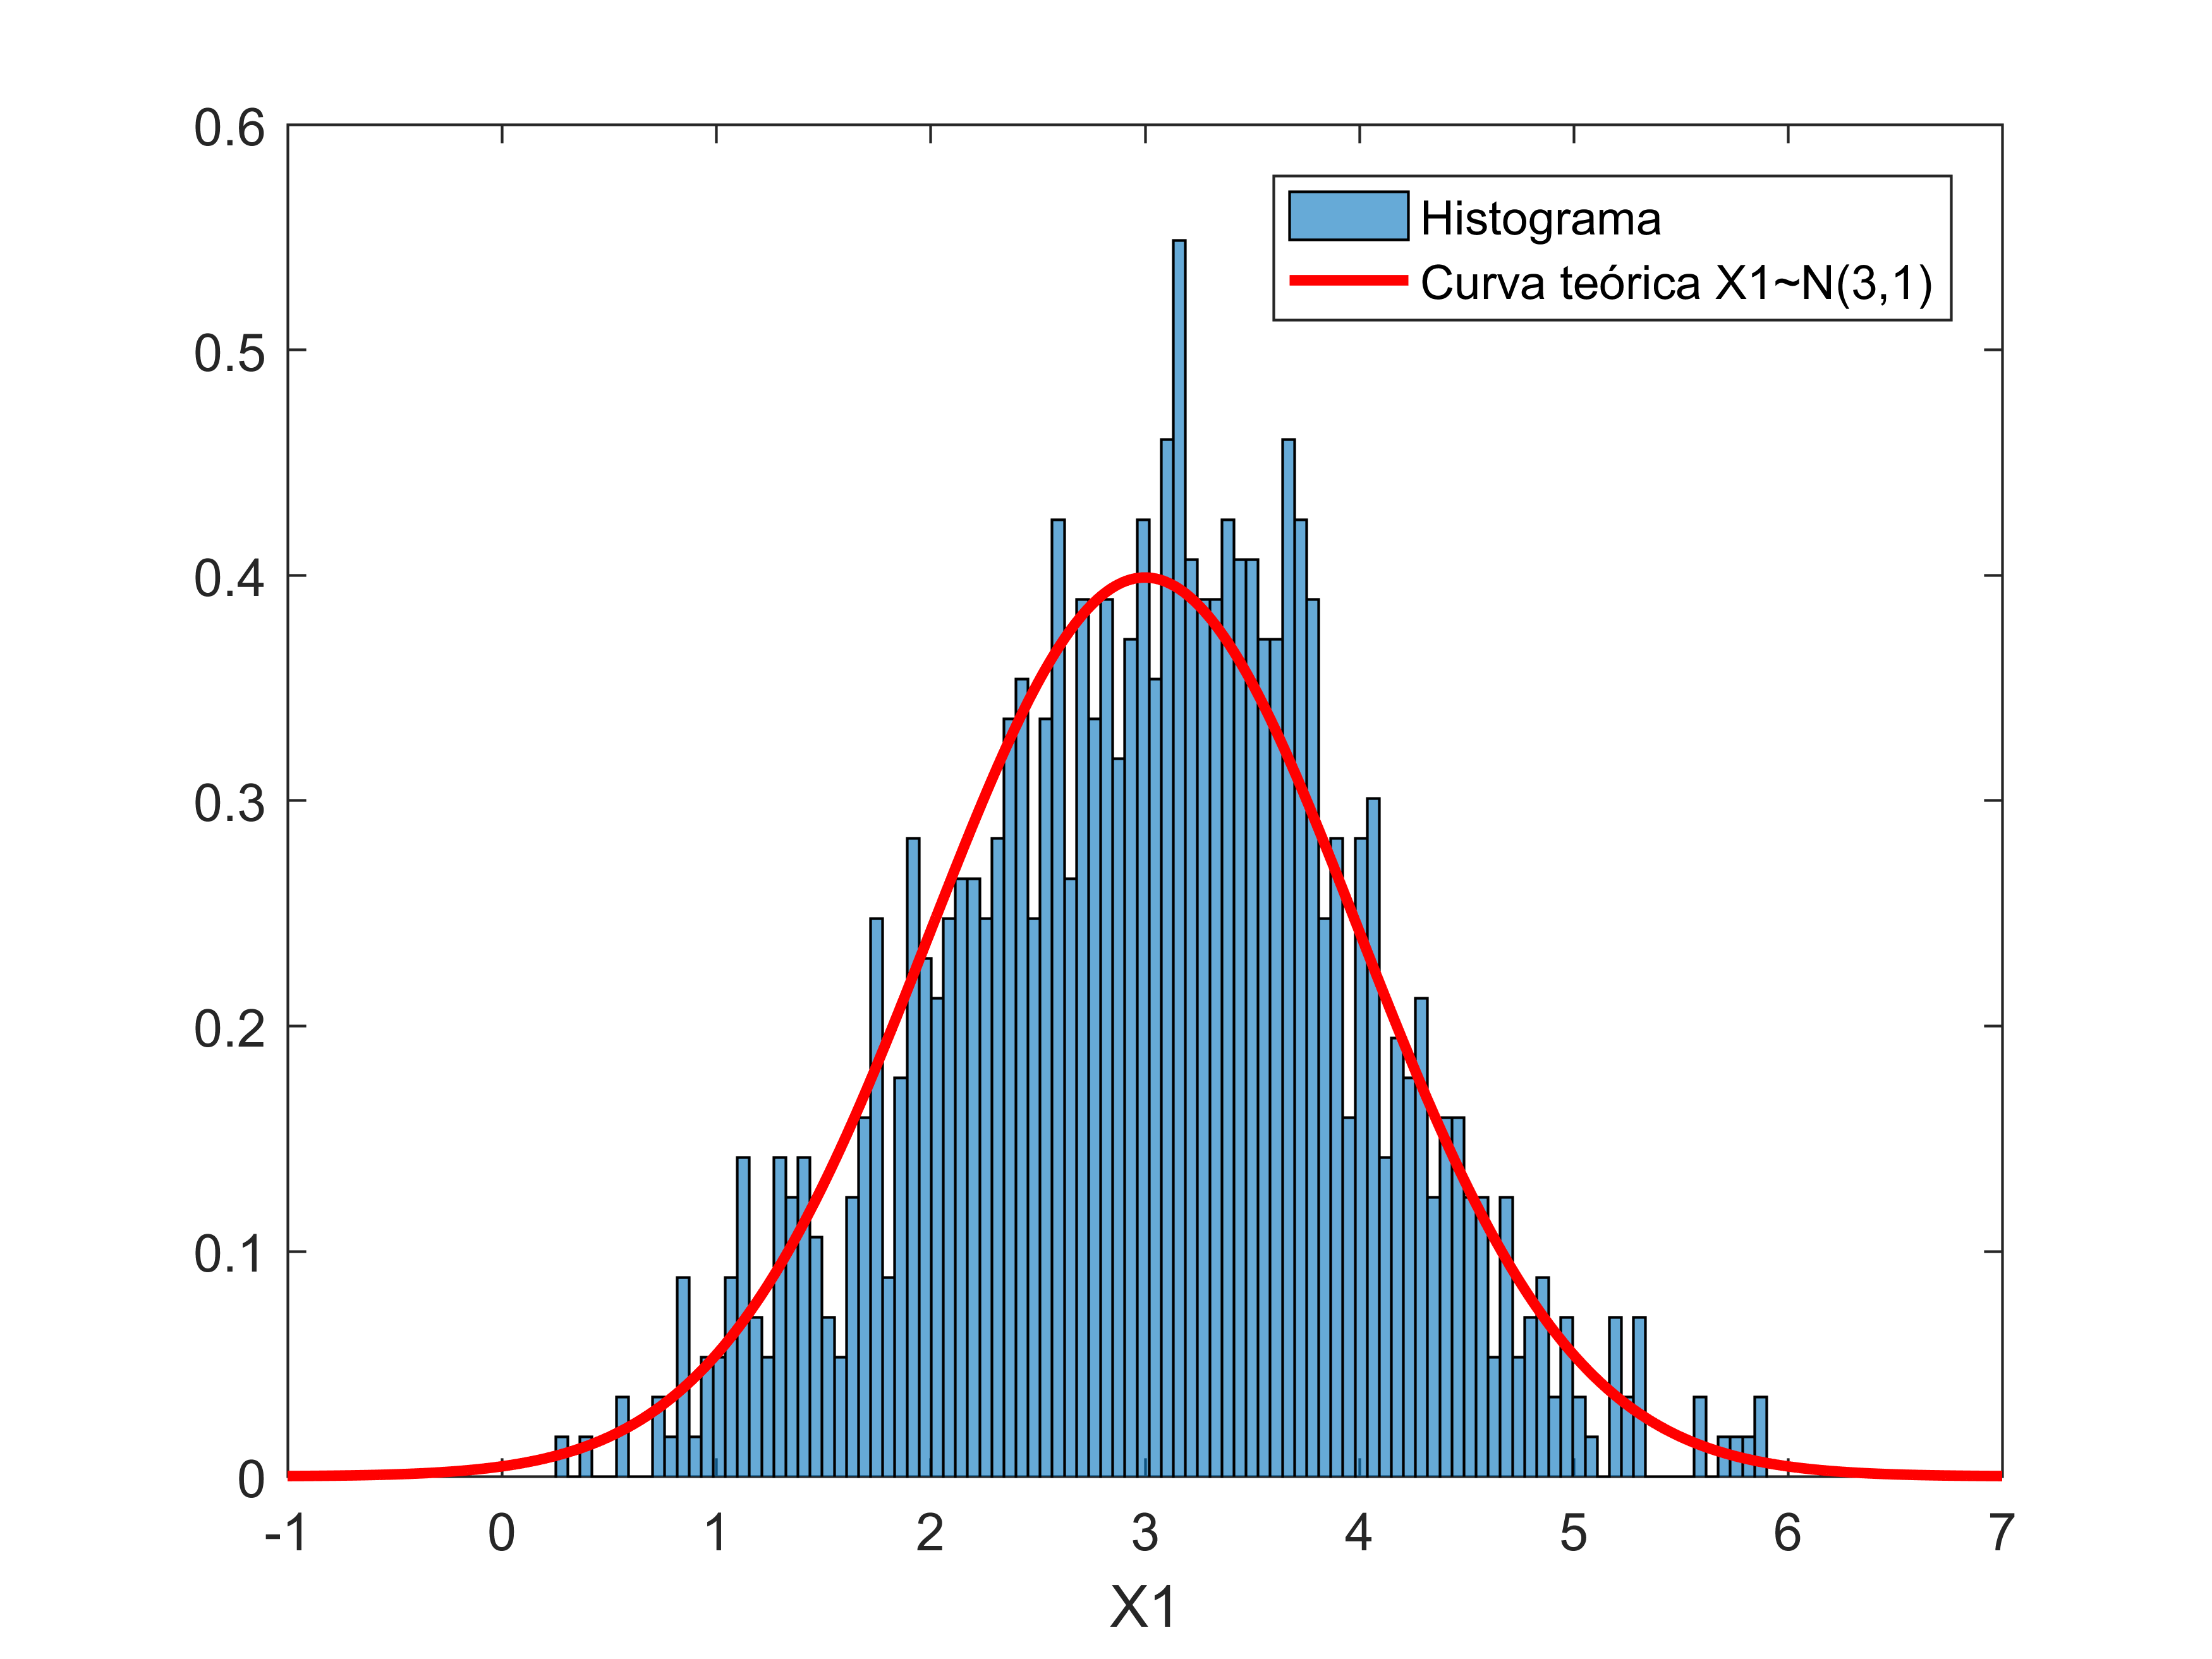
\includegraphics[scale=0.55]{Imagenes/X1_1000.png}
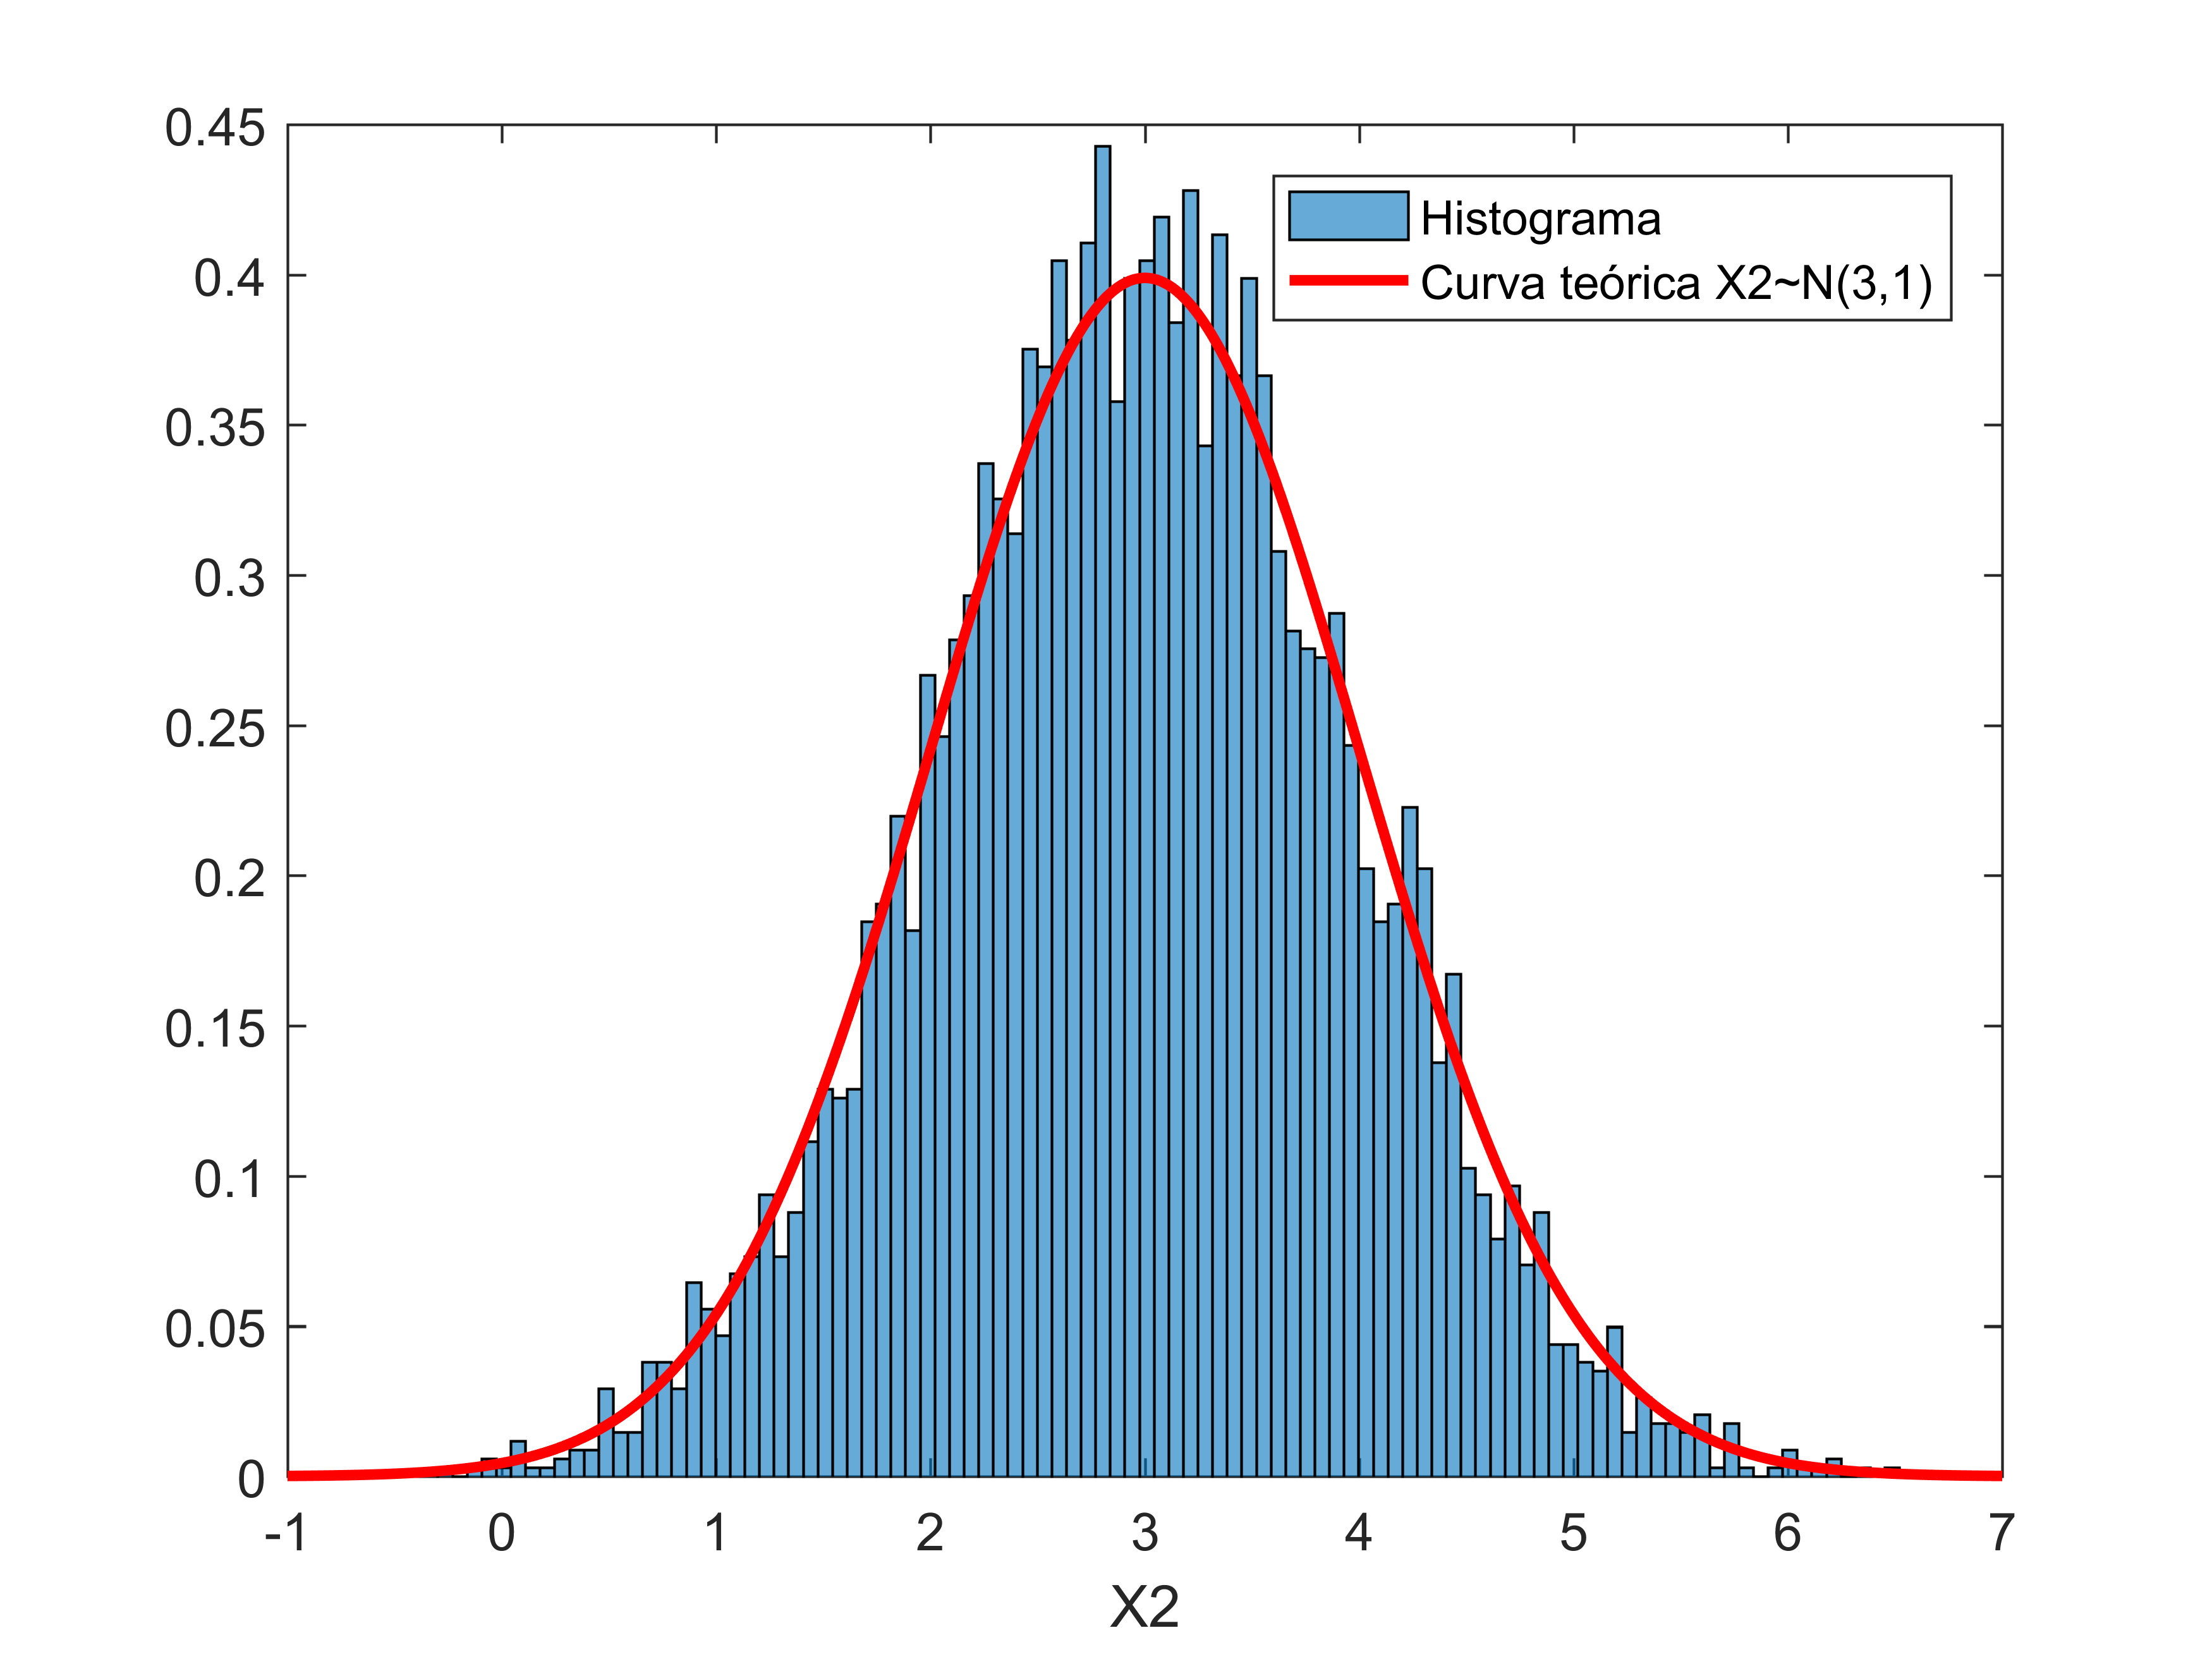
\includegraphics[scale=0.55]{Imagenes/X2_5000.png}
\par\end{centering}
\caption{Comparación para vectores $X_1$ de 1000 elementos e $X_2$ de 5000 elementos}

\end{figure} 

\newpage

\begin{figure}[!ht]
\begin{centering}
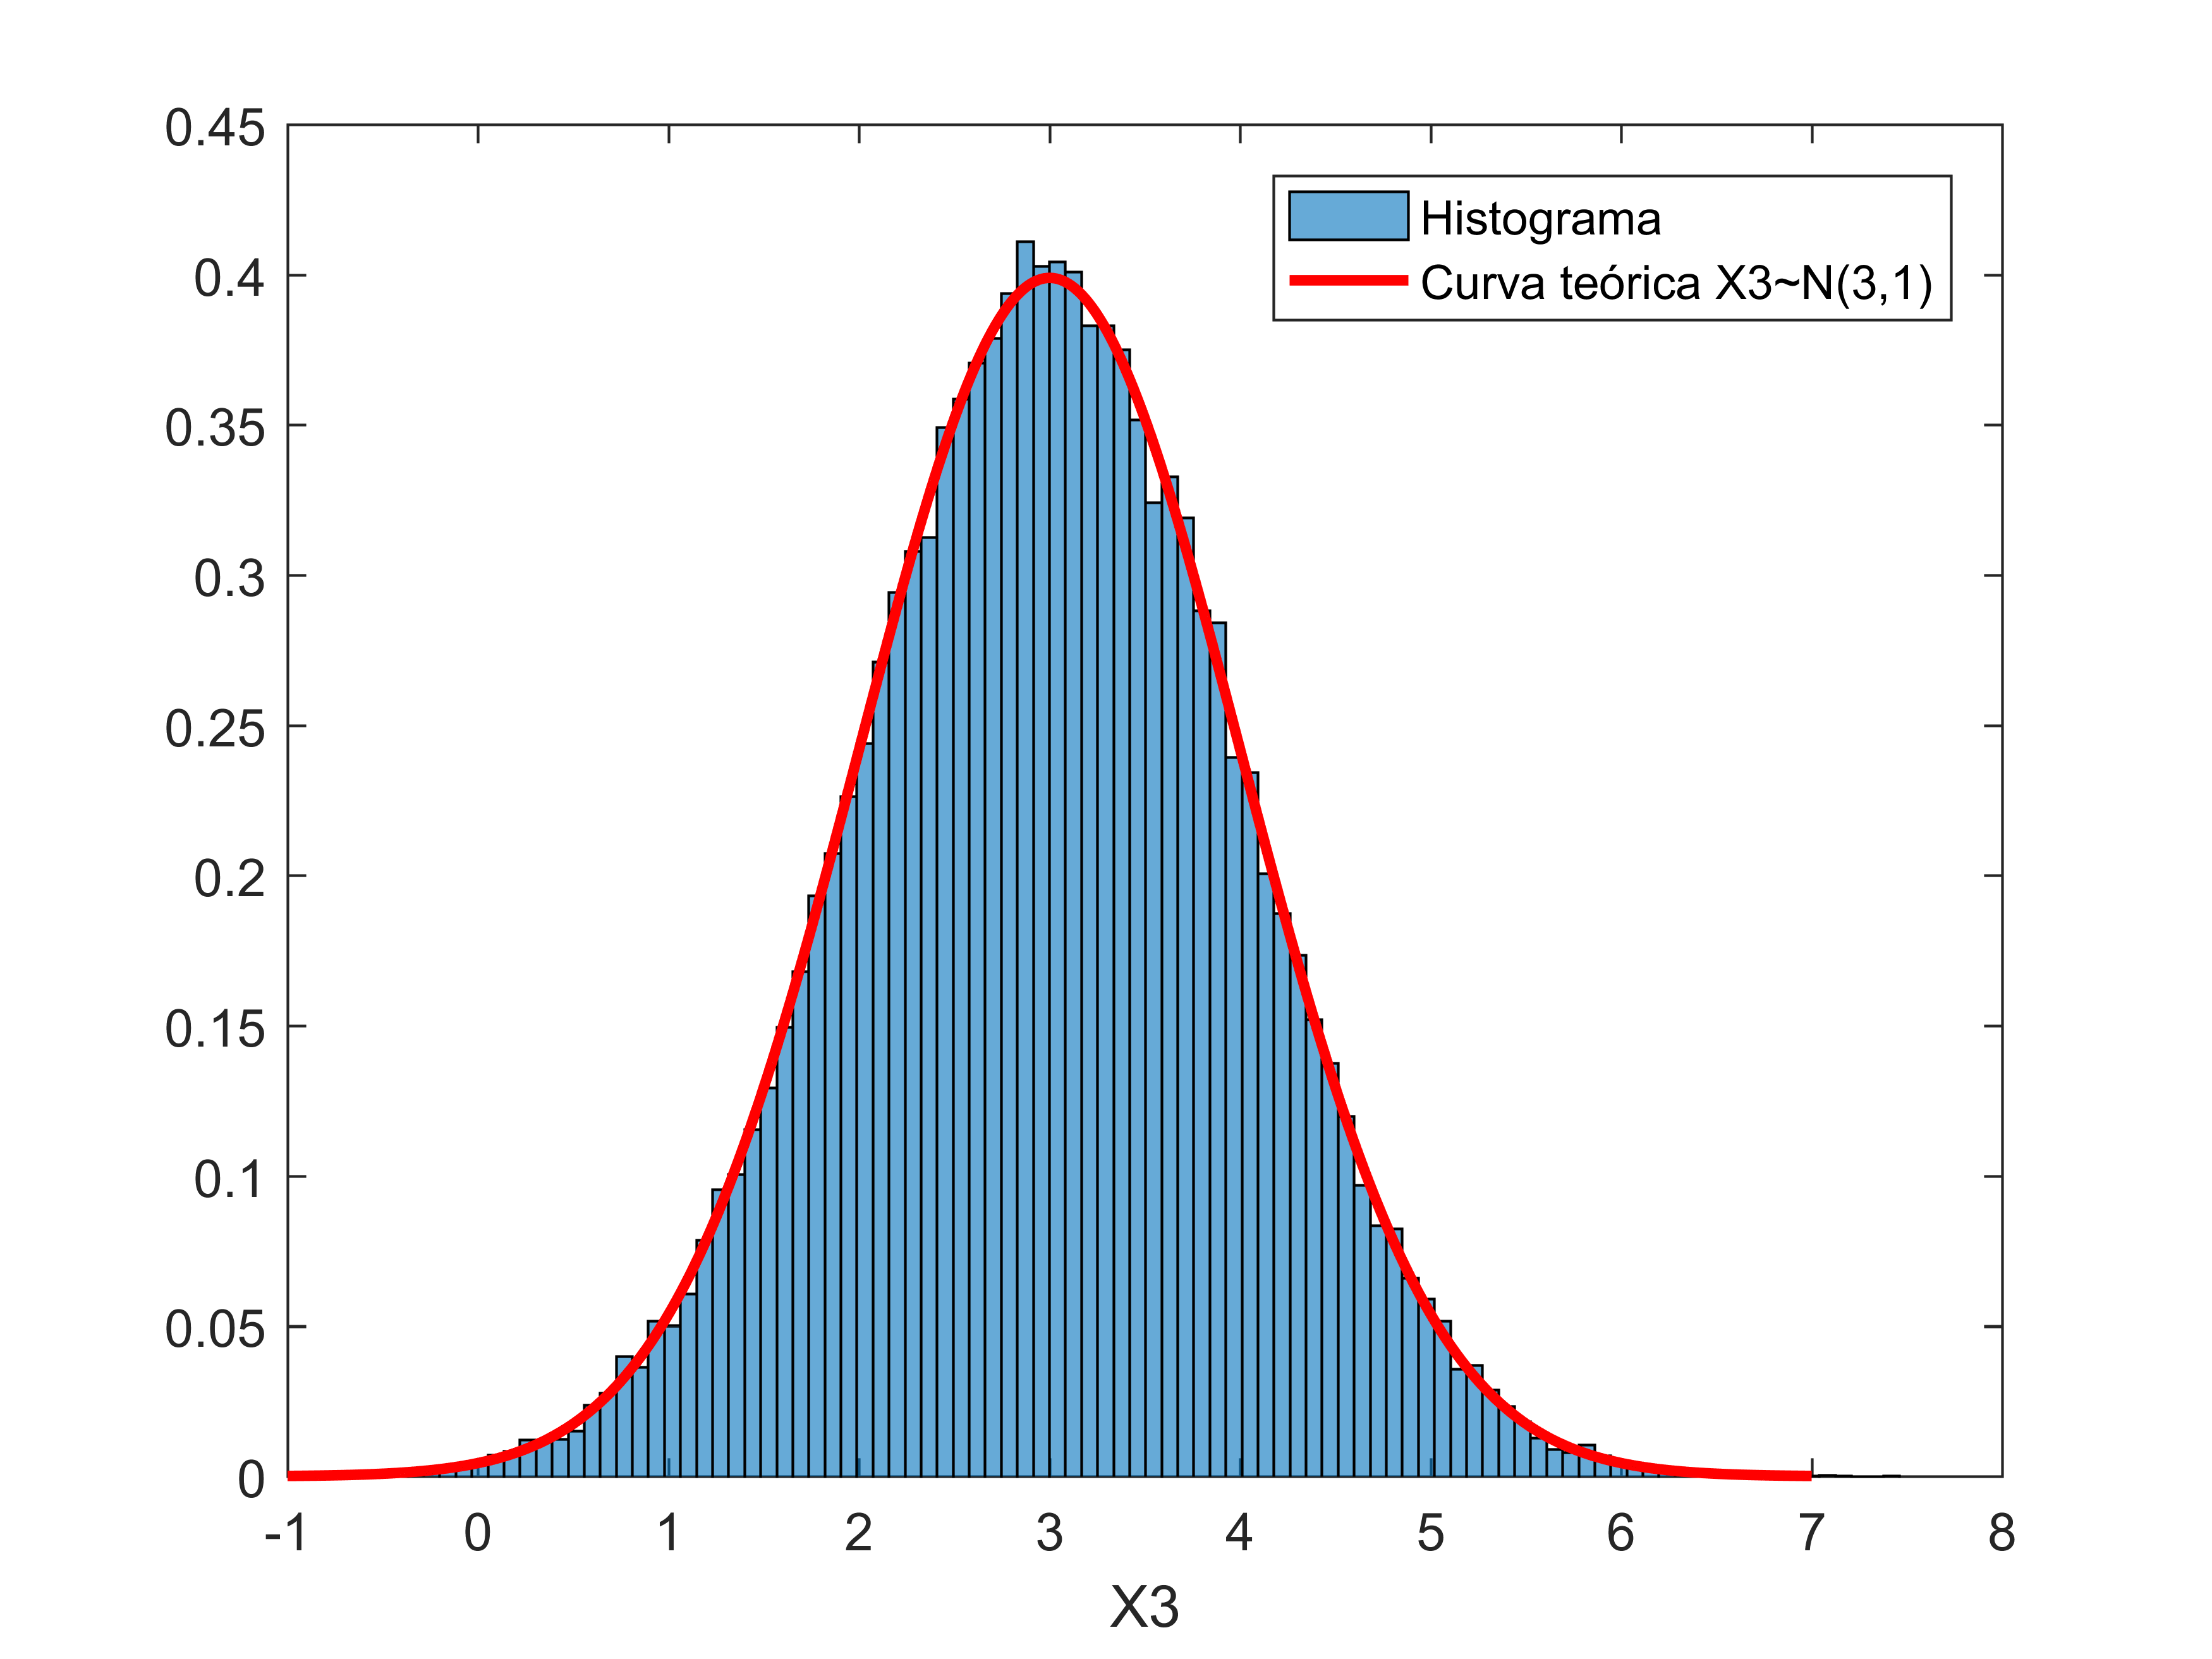
\includegraphics[scale=0.55]{Imagenes/X3_50000.png}
\par\end{centering}
\caption{Comparación para vector $X_3$ de 50000 elementos}

\end{figure} 

Utilizando un n\'umero fijo de barras adecuado, se consigue el ajuste mostrado en las gr\'aficas anteriores. Para mayor cantidad de elementos, el histograma tiende a parecerse m\'as a la curva de la gaussiana te\'orica.\par
El c\'odigo de MatLab utilizado para la simulaci\'on se muestra a continuaci\'on.

\lstinputlisting[language=Matlab, caption=Codigo de implementaci\'on]{Codigos/ItemAB.m}

\subsection{Valores de $\mu$ y $\sigma^2$ te\'oricas con estimadas}

De los vectores anteriores se estima la media y la varianza para cada caso, comparando con los te\'oricos en el siguiente cuadro.

\begin{table}[!ht]
\begin{centering}

\begin{tabular}{|c||c|c|c||c|c|c|}
\hline 
\multirow{2}{*}{Elementos} & \multicolumn{3}{c||}{$\mu_x$} & \multicolumn{3}{c|}{$\sigma^2_x$}\tabularnewline
\cline{2-7} 
 & Te\'orico & Estimado & $\Delta \mu_x$ & Te\'orico & Estimado & $\Delta \sigma^2_x$ \\
\hline 
\hline 
1000 & 3 & 3.0402 & 0.0402 & 1 & 0.9348 & 0.0652\\
\hline 
5000 & 3 & 2.9882 & 0.0118 & 1 & 0.9577 & 0.0423\\
\hline 
50000 & 3 & 3.0006 & 0.0006 & 1 & 0.9984 & 0.0016\\
\hline 
\end{tabular}
\par\end{centering}
\caption{Valores estimados y te\'oricos}

\end{table}

Dado que el n\'umero de elementos es bastante grande en los casos analizados, los valores estimados caen siempre muy cerca de los te\'oricos. A mayor cantidad de elementos la diferencia entre el valor te\'orico y el estimado tiende a ser menor.

\subsection{Estimaciones de $\mu_x$ - Histograma}

Para este caso, se realizan 10000 estimaciones en distribuciones con 10000 elementos cada una. El c\'odigo de MatLab utilizado para la simulaci\'on es el siguiente.

\lstinputlisting[language=Matlab, caption=C\'odigo de implementaci\'on]{Codigos/ItemD.m}

\newpage

Realizando un histograma de los valores obtenidos, se tiene:

\begin{figure}[!ht]
\begin{centering}
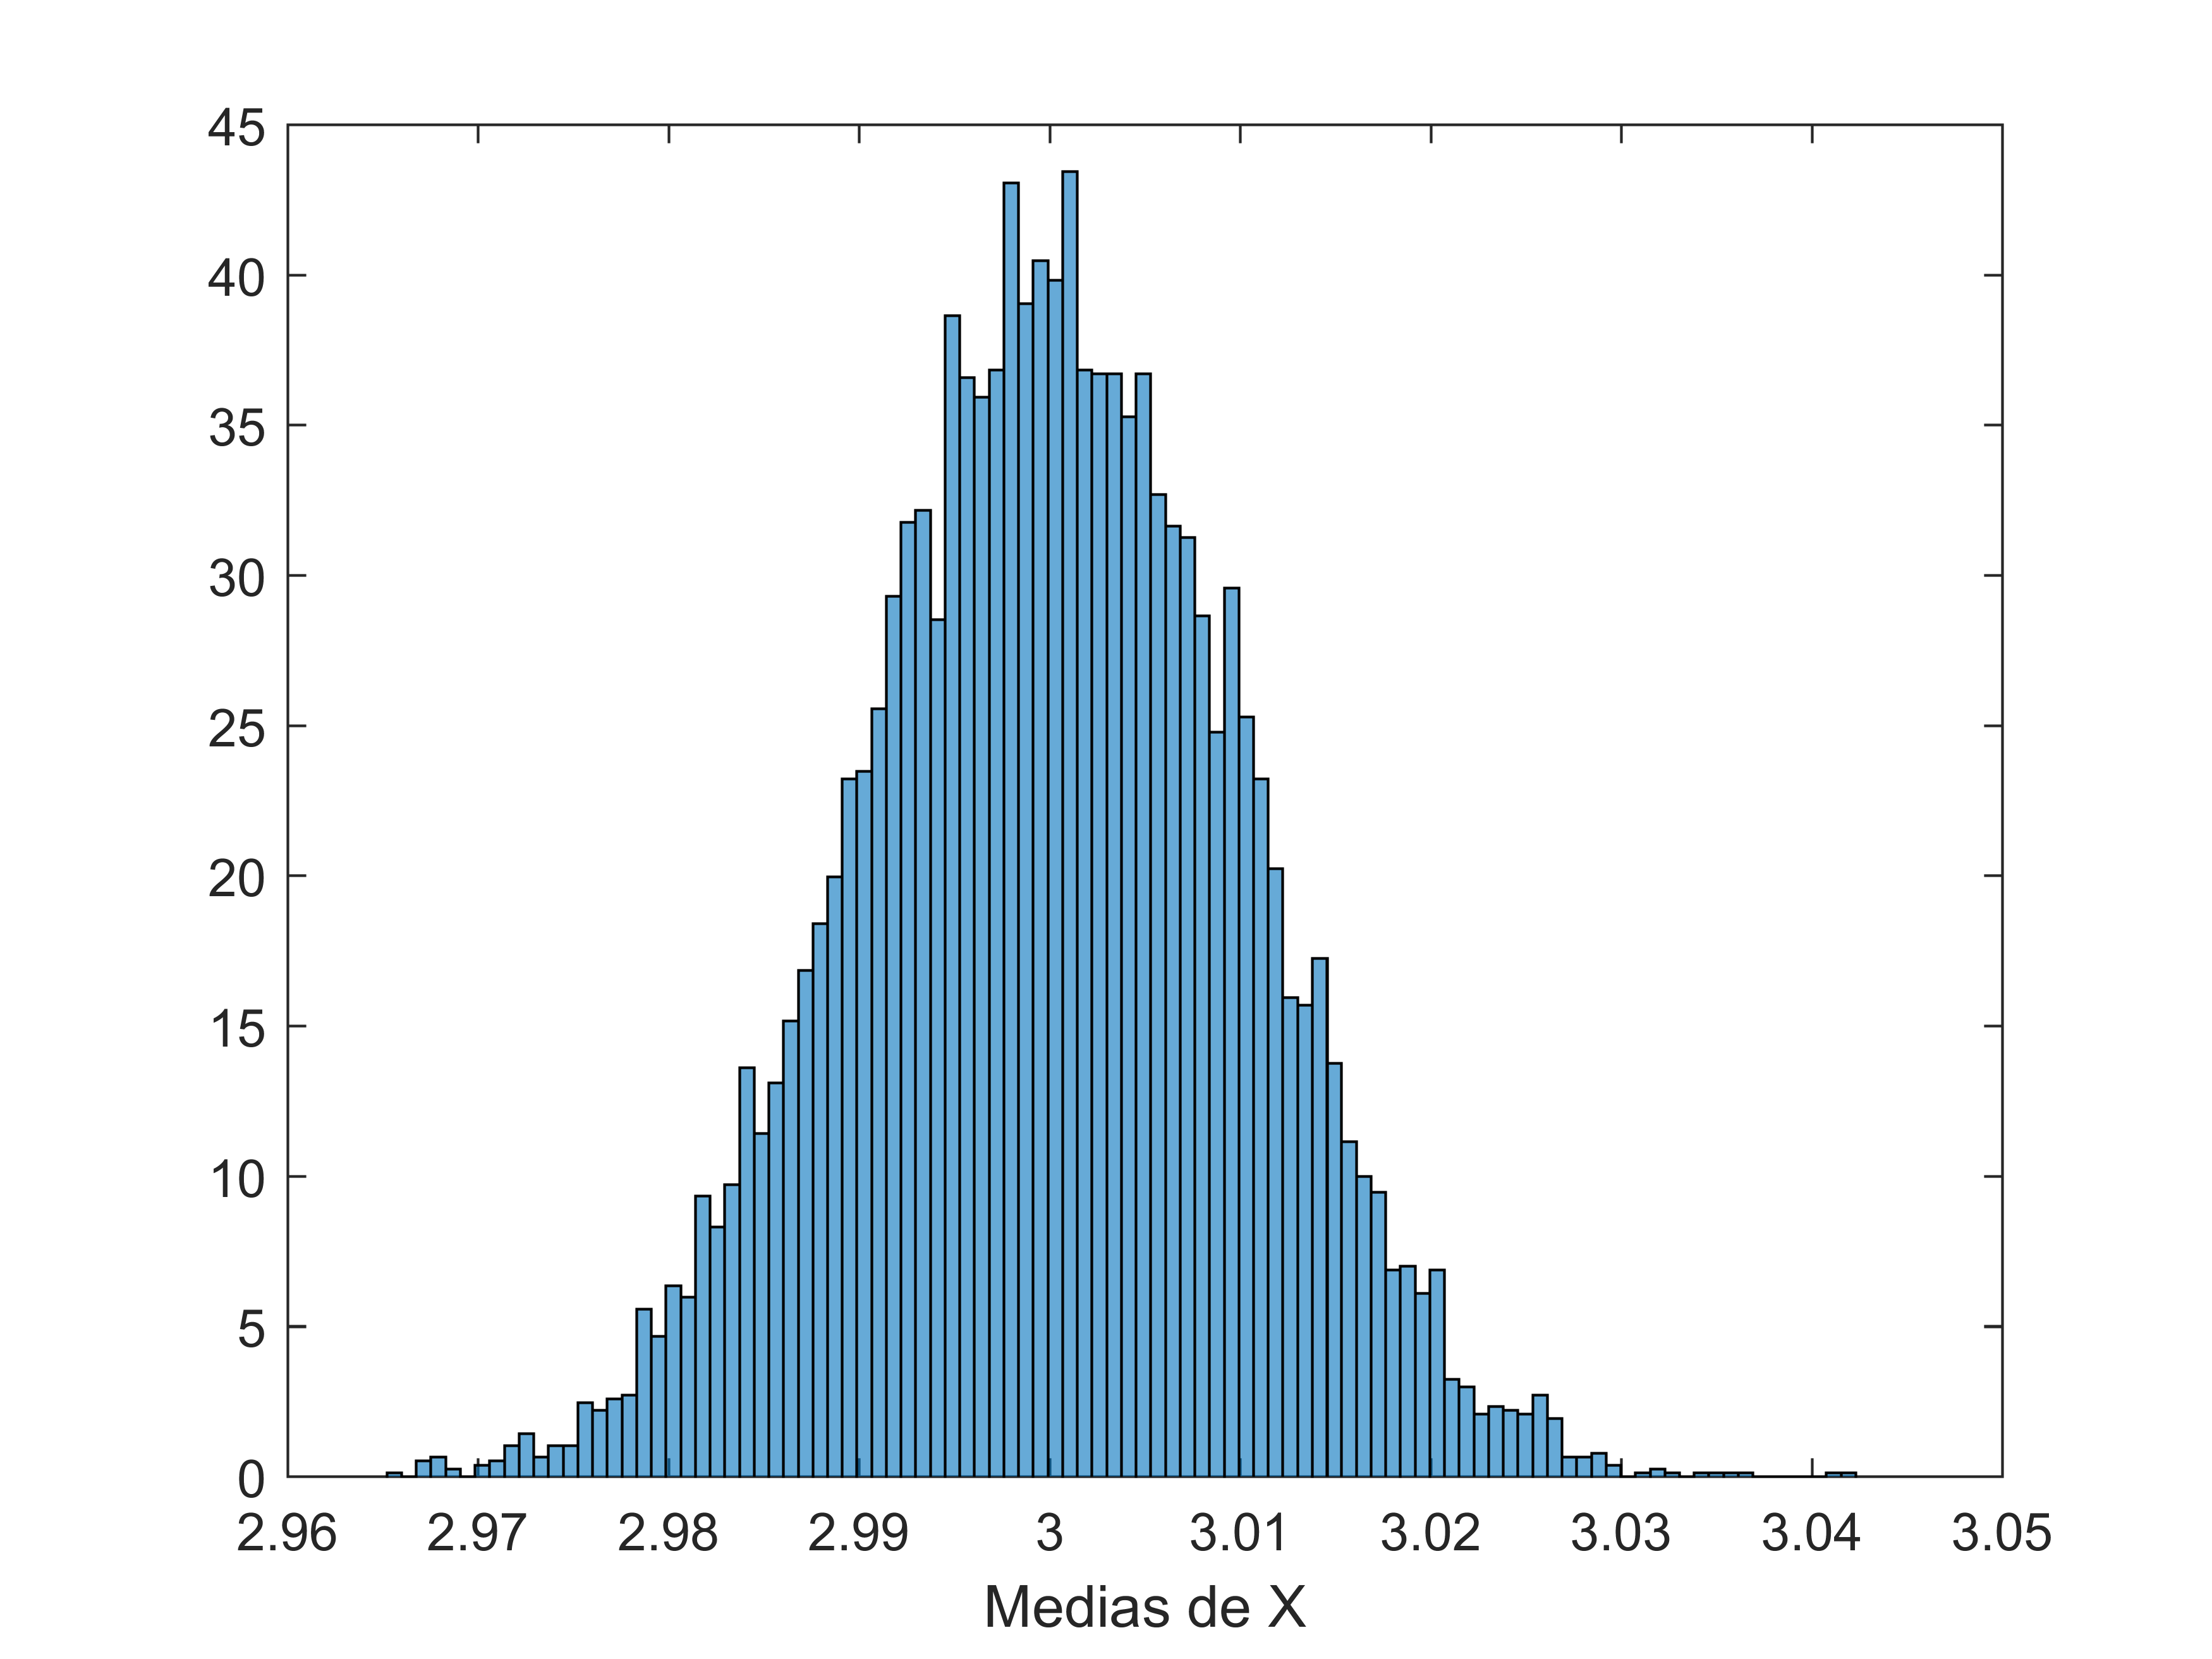
\includegraphics[scale=0.55]{Imagenes/MediasX.png}
\par\end{centering}
\caption{Histograma de las medias estimadas, con resultante $\mu = 3.0001$ - $\sigma = 0.01$}

\end{figure} 

Si llamamos a la media estimada $m_X$, se la define en este caso como:

\[
m_X = \frac{1}{N} \cdot \sum^N_{i=1} \mu_{X_i} \hspace{2cm} \textrm{Con N = 10000} 
\]

Como la distribuci\'on normal es reproductiva, la suma de N variables aleatorias con dicha distribuci\'on resulta tambi\'en normal. Esto \'ultimo tambi\'en puede verse desde el Teorema Central del L\'imite, dado que el valor de N utilizado es suficientemente grande. Para el caso en cuesti\'on, los valores te\'oricos de $\mu$ y $\sigma$ son:

\[
E(m_X) = \mu = \frac{1}{N} \cdot \underbrace{\sum^N_{i=1} E(\mu_{X_i})}_{\textrm{Por linealidad}} = \frac{1}{N} \cdot \sum^N_{i=1} \mu_x = \mu_x \Longrightarrow \mu = 3
\]

\[
\sigma^2(m_X) = \sigma^2 = \frac{1}{N^2} \cdot \underbrace{\sum^N_{i=1} \sigma^2(\mu_{X_i})}_{\textrm{Por independencia}} = \frac{1}{N^2} \cdot \sum^N_{i=1} \sigma^2_x = \frac{\sigma^2_x}{N} \Longrightarrow \sigma = 0.0001
\]

De donde se observa que los valores estimados sobre la media del vector graficado en el histograma resultan muy cercanos a los te\'oricos.

\subsection{Error en la estimaci\'on de $\mu_x$ - Ejemplo}

Se toma ahora un caso particular, donde la cantidad de elementos (vectores con $K$ n\'umeros aleatorios con distribuci\'on normal) es desconocida, y se busca que la probabilidad de que el valor estimado $m_X$ se aparte m\'as del 4\% del valor te\'orico sea menor al 2\%. Es decir:

\[
P[|m_X - \mu_x| > 0.04\mu_x] \leq 0.02
\]

Se utiliza un $K$ lo suficientemente grande para considerar que los vectores $X$ tienen media $\mu_x$ y desv\'io est\'andar $\sigma_x$ iguales a los te\'oricos con los que se generaron los n\'umeros aleatorios que \'estos contienen. Si se trabaja con la expresi\'on:

\[
2 \cdot P[m_X - \mu_x < -0.04\mu_x] \leq 0.02
\]
\[
P\left[\left( \frac{m_X - \mu_x}{\sigma_x} \right) \cdot \sqrt{N} < -0.04 \cdot \frac{\mu_x}{\sigma_x} \cdot \sqrt{N}\right] \leq 0.01
\]

La variable aleatoria $\left( \dfrac{m_X - \mu_x}{\sigma_x} \right) \cdot \sqrt{N}$ tiene distribuci\'on normal est\'andar. La llamamos $\Phi$:

\[
\Phi \left( -0.04 \cdot \frac{\mu_x}{\sigma_x} \cdot \sqrt{N} \right) \leq 0.01
\]
\[
\Phi \left( 0.04 \cdot \frac{\mu_x}{\sigma_x} \cdot \sqrt{N} \right) \geq 0.99
\]
\[
0.04 \cdot \frac{\mu_x}{\sigma_x} \cdot \sqrt{N} \geq \Phi^{-1}(0.99) \approx 2.3263
\]
\[
N \geq 3382.3 \cdot \frac{\sigma^2_x}{\mu^2_x}
\]

Para el caso analizado, $\mu_x = 3$ y $\sigma^2_x = 1$:

\[
N \geq 375.9
\]

El c\'odigo utilizado para verificar por simulaci\'on es el siguiente:

\lstinputlisting[language=Matlab, caption=C\'odigo de implementaci\'on]{Codigos/ItemE.m}

Donde la probabilidad P calculada efectivamente resulta $\leq 0.02$.

\newpage

\section{Variables aleatorias conjuntamente gaussianas}

En este caso se analizan dos variables aleatorias conjuntamente gaussianas, cuyos par\'ametros son:

\begin{table}[ht]
\begin{centering}
\begin{tabular}{|c||c|c|c|c|c|}
\hline 
Caso & $\mu_x$ & $\mu_y$ & $\sigma_x$ & $\sigma_y$ & $\rho$\\
\hline 
\hline 
A & 2 & 3 & 1 & 1 & -0.5\tabularnewline
\hline 
B & 2 & 3 & 1 & 0.5 & -0.8\tabularnewline
\hline 
\end{tabular}
\par\end{centering}
\caption{Par\'ametros para los casos analizados}

\end{table}

Las variables $X_n$ con distribuci\'on normal est\'andar son generadas utilizando el m\'etodo de simulaci\'on de montecarlo (mediando dos variables aleatorias con distribuci\'on uniforme al igual que antes), y mediante la transformaci\'on lineal siguiente se halla la variable $X$:

\[
X = \sigma_x X_n + \mu_x
\]

An\'alogamente se halla la variable $Y$:

\[
Y = \sigma_y Y_n + \mu_y
\]

Para dibujar la nube de puntos con ambas variables se tiene la funci\'on de densidad de probabilidad gaussiana bivariable:

\[
f_{XY}(x,y) = \frac{1}{2 \pi \sigma_x \sigma_y \sqrt{1-\rho^2}} e^{- \frac{1}{2 \left(1-\rho^2\right)} \left[ \left( \frac{x-\mu_x}{\sigma_x} \right)^2 + \left( \frac{y-\mu_y}{\sigma_y} \right)^2 - \frac{2 \rho (x-\mu_x) (y-\mu_y)}{\sigma_x \sigma_y} \right]}
\]

Teniendo los elementos anteriores, se implementa el siguiente c\'odigo en MatLab para obtener los gr\'aficos resultantes.

\lstinputlisting[language=Matlab, caption=C\'odigo de implementaci\'on]{Codigos/EJ2.m}

Los resultados obtenidos para ambos casos se muestran a continuaci\'on.

\begin{figure}[!ht]
\begin{centering}
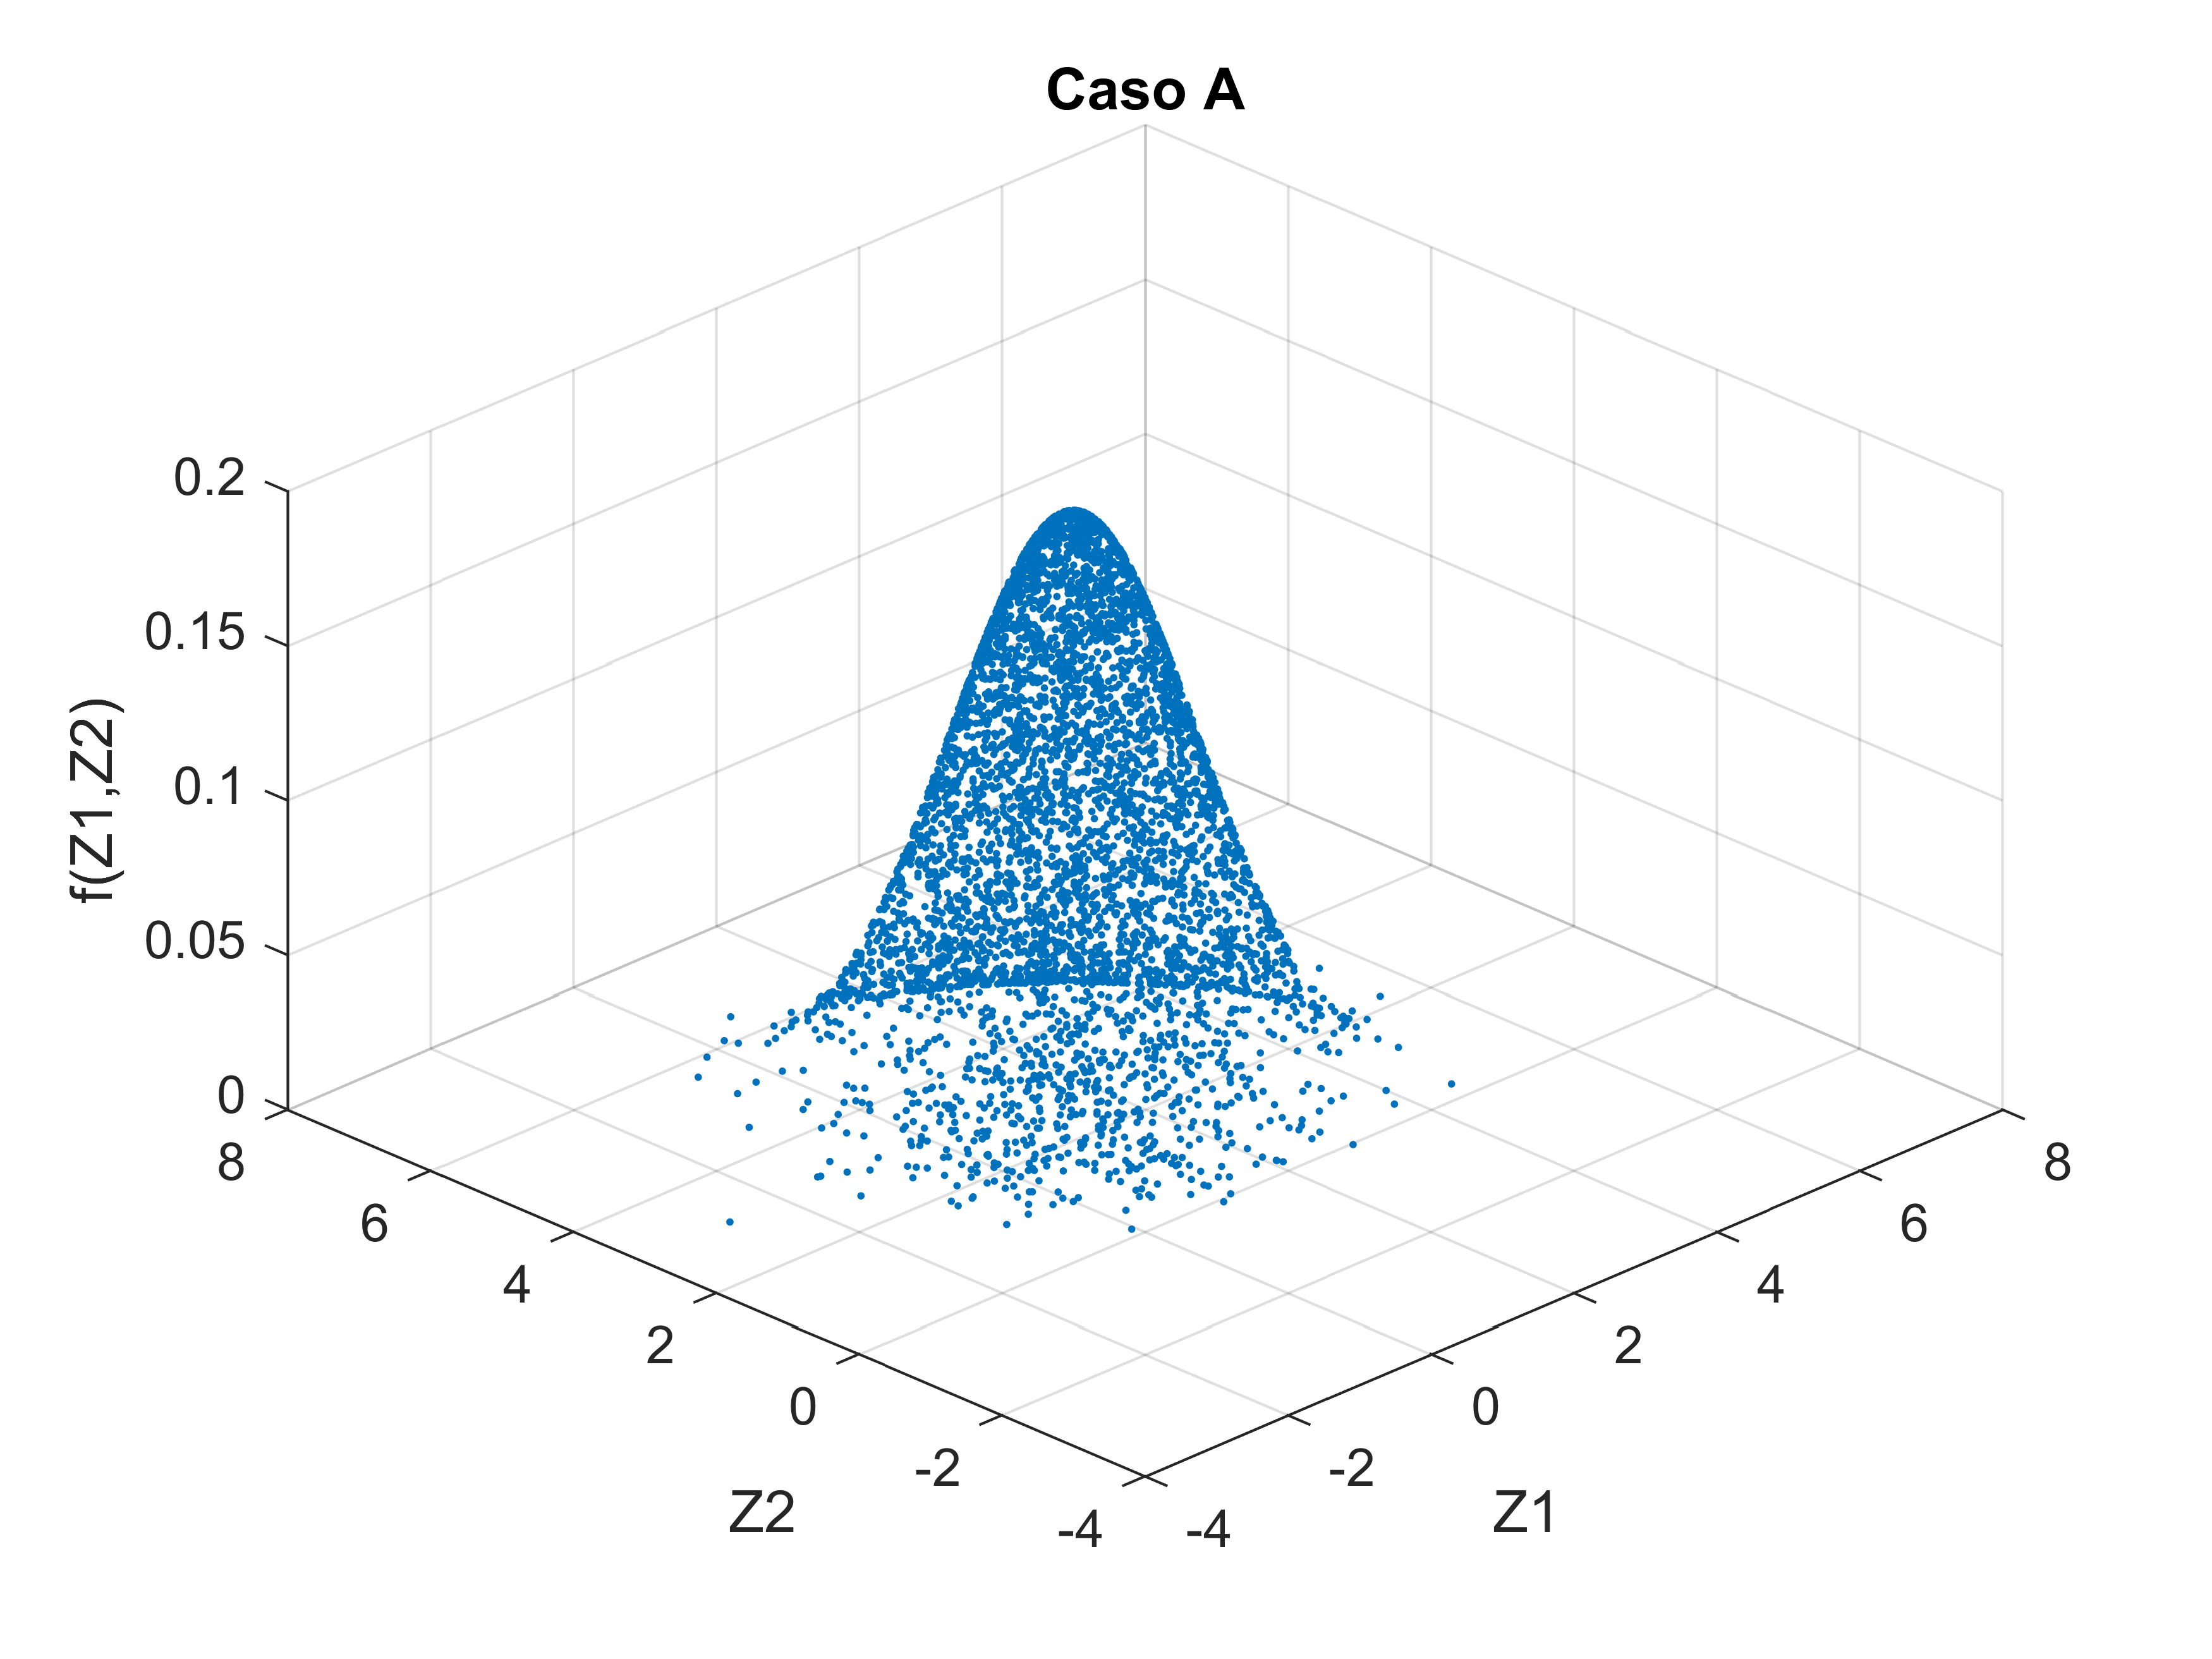
\includegraphics[scale=0.55]{Imagenes/Za.png}
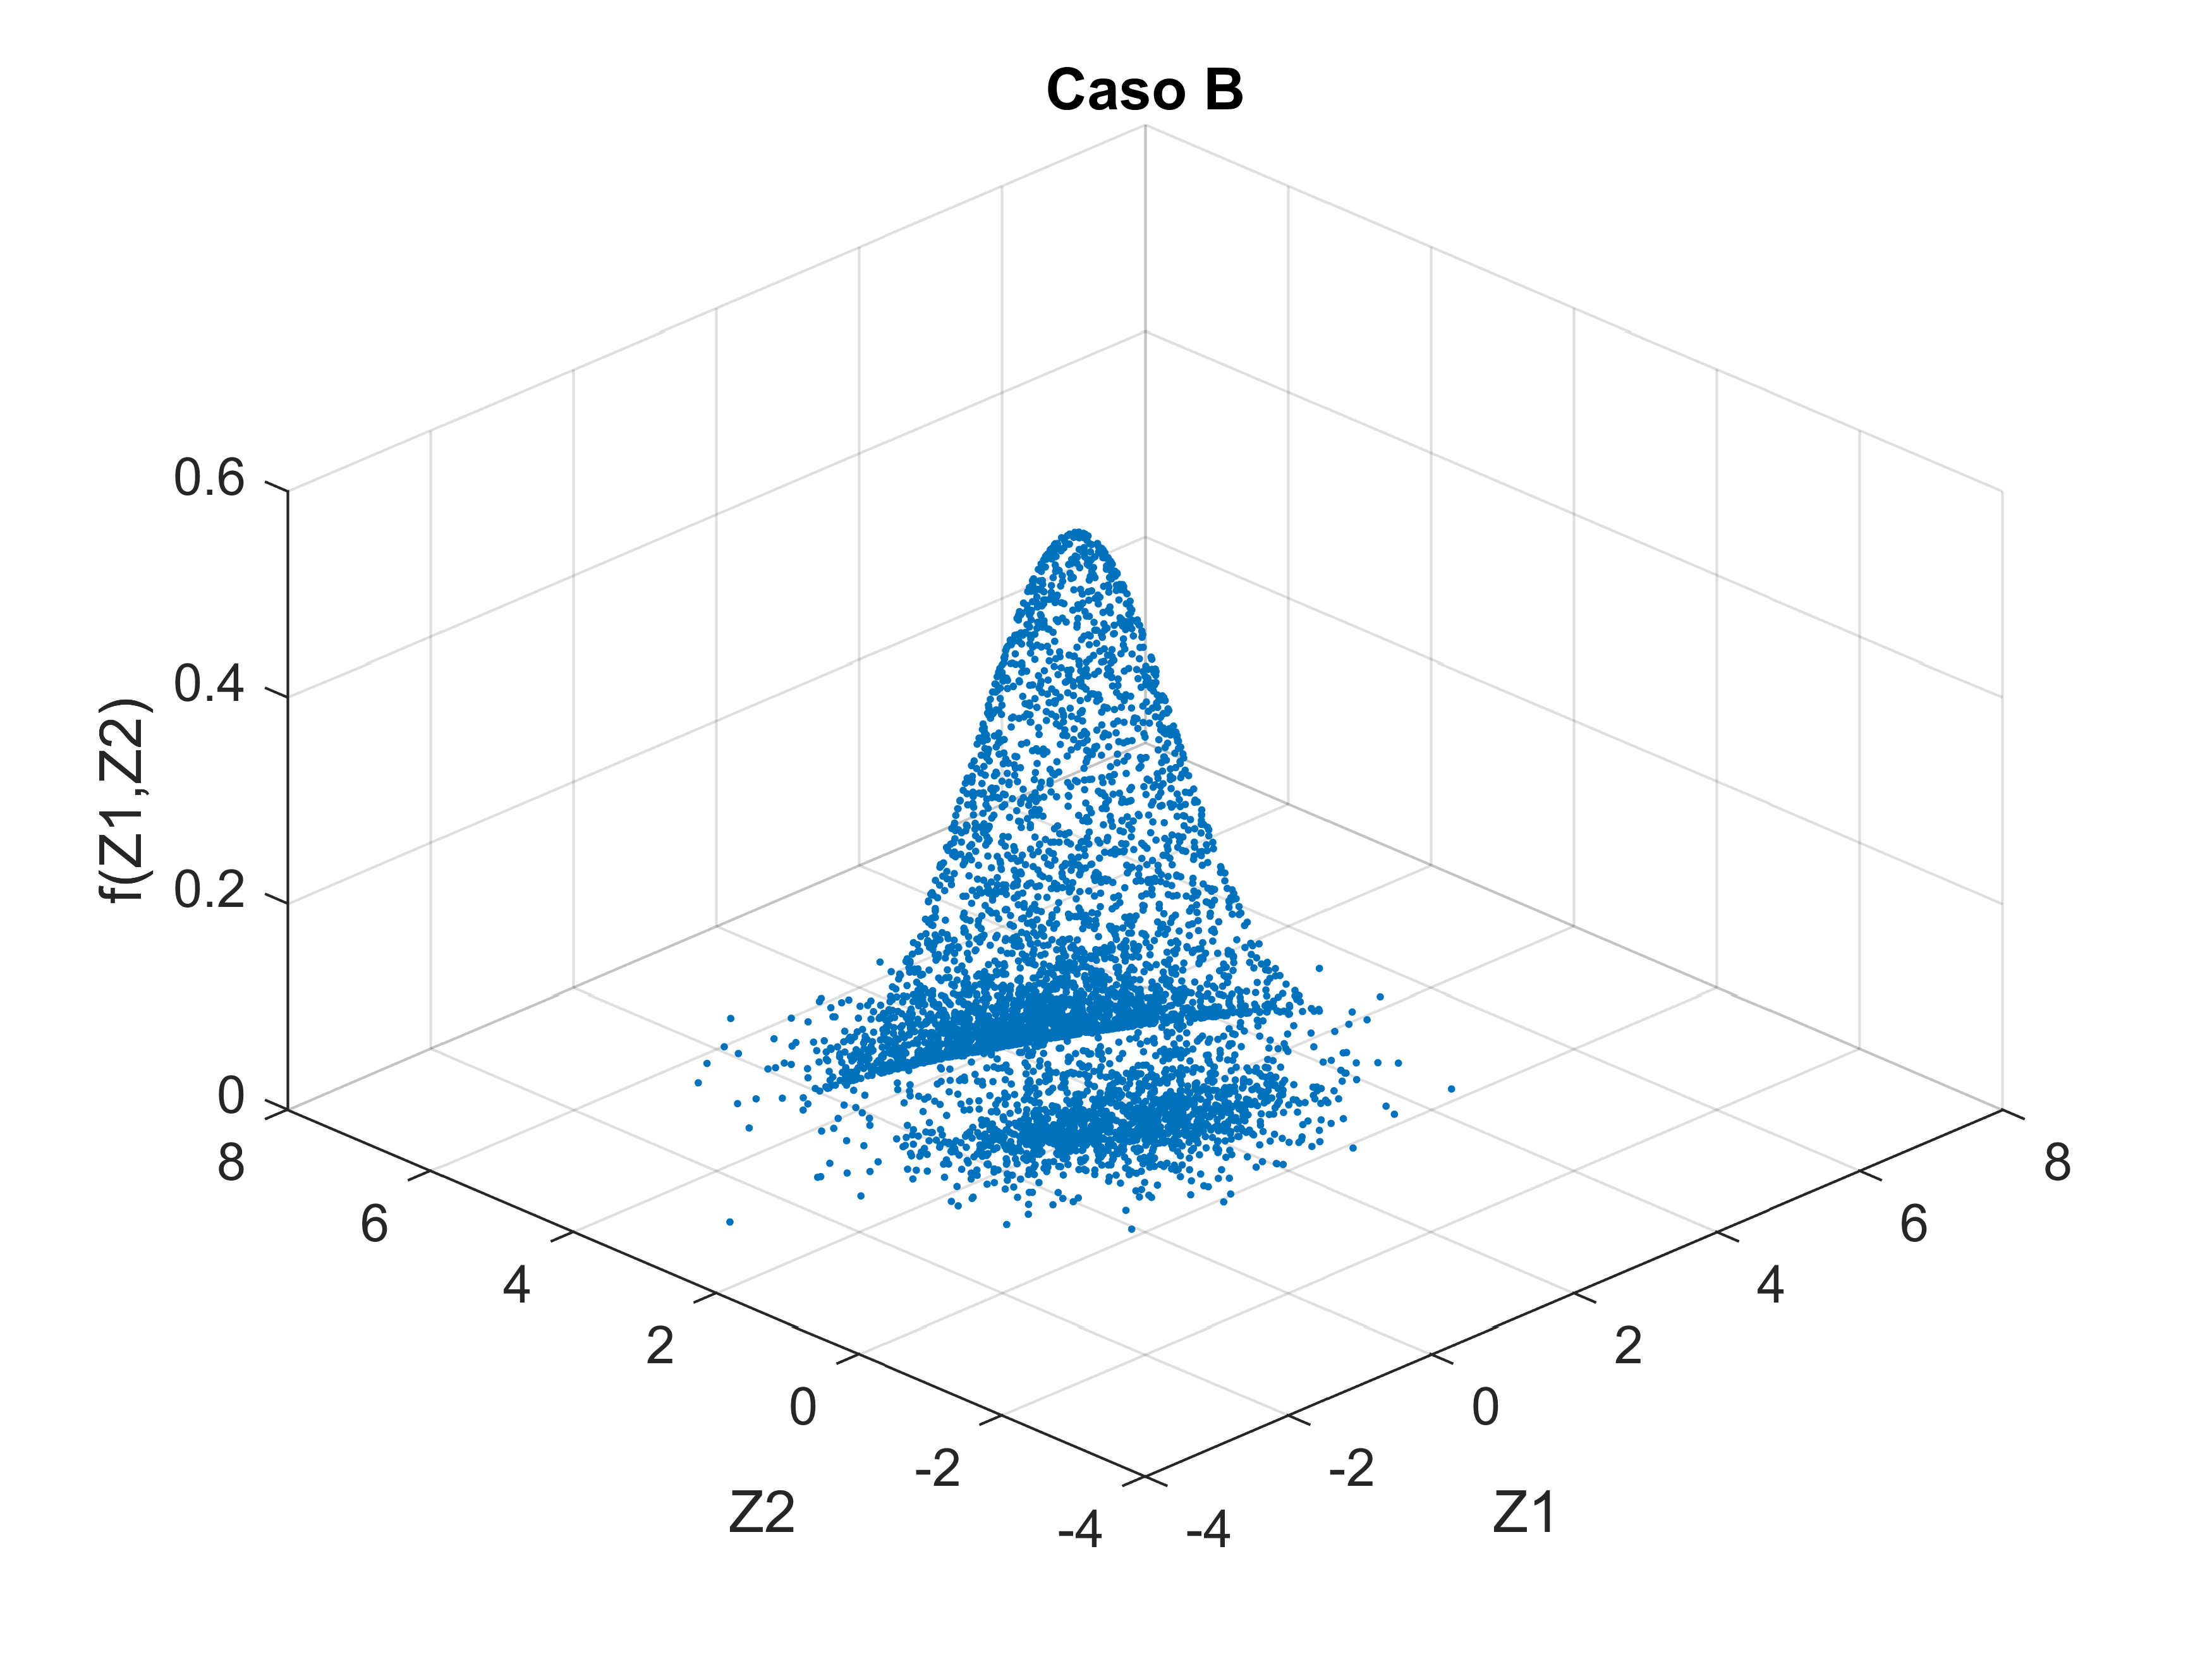
\includegraphics[scale=0.55]{Imagenes/Zb.png}
\par\end{centering}
\caption{Nube de puntos resultante para ambos casos}

\end{figure} 

Para el caso A, se tiene que $\sigma_x = \sigma_y$, por lo que si se realizan las curvas de nivel se observar\'ian c\'irculos, donde la orientaci\'on de sus ejes est\'a dada por el coeficiente de correlaci\'on $\rho$. En el caso B, se tiene $\sigma_x \neq \sigma_y$, por lo que las curvas de nivel resultantes son elipses. El $|\rho|$ es mayor que en el caso anterior, por lo que la orientaci\'on de sus ejes resulta distinta. Se observa que a medida que el $|\rho| \longrightarrow 1$, las elipses se van 'estirando', hasta que en el l\'imite tiende a una recta.\par
En dicho l\'imite, se tiene una relaci\'on directamente lineal entre $X$ e $Y$, por lo que conociendo cu\'anto vale uno ya se conoce el otro, mediante:

\[
y = \frac{\sigma_y}{\sigma_x}x + \mu_y - \frac{\sigma_y}{\sigma_x} \mu_x
\] 

\newpage

\section{Proceso de Poisson}

El proceso aleatorio asignado en este caso es el proceso de Poisson. Se utiliza un contador $Q(t)$, que indica el n\'umero de eventos ocurridos hasta el tiempo $t$.\par
El c\'odigo utilizado para generar las funciones muestra se detalla a continuaci\'on. Se ajust\'o de manera tal que la media $\lambda t$ tenga $\lambda \approx 1$.

\lstinputlisting[language=Matlab, caption=C\'odigo de implementaci\'on]{Codigos/EJ3A.m}

En lo que sigue se plasman algunas funciones muestra generadas.

\begin{figure}[!ht]
\begin{centering}
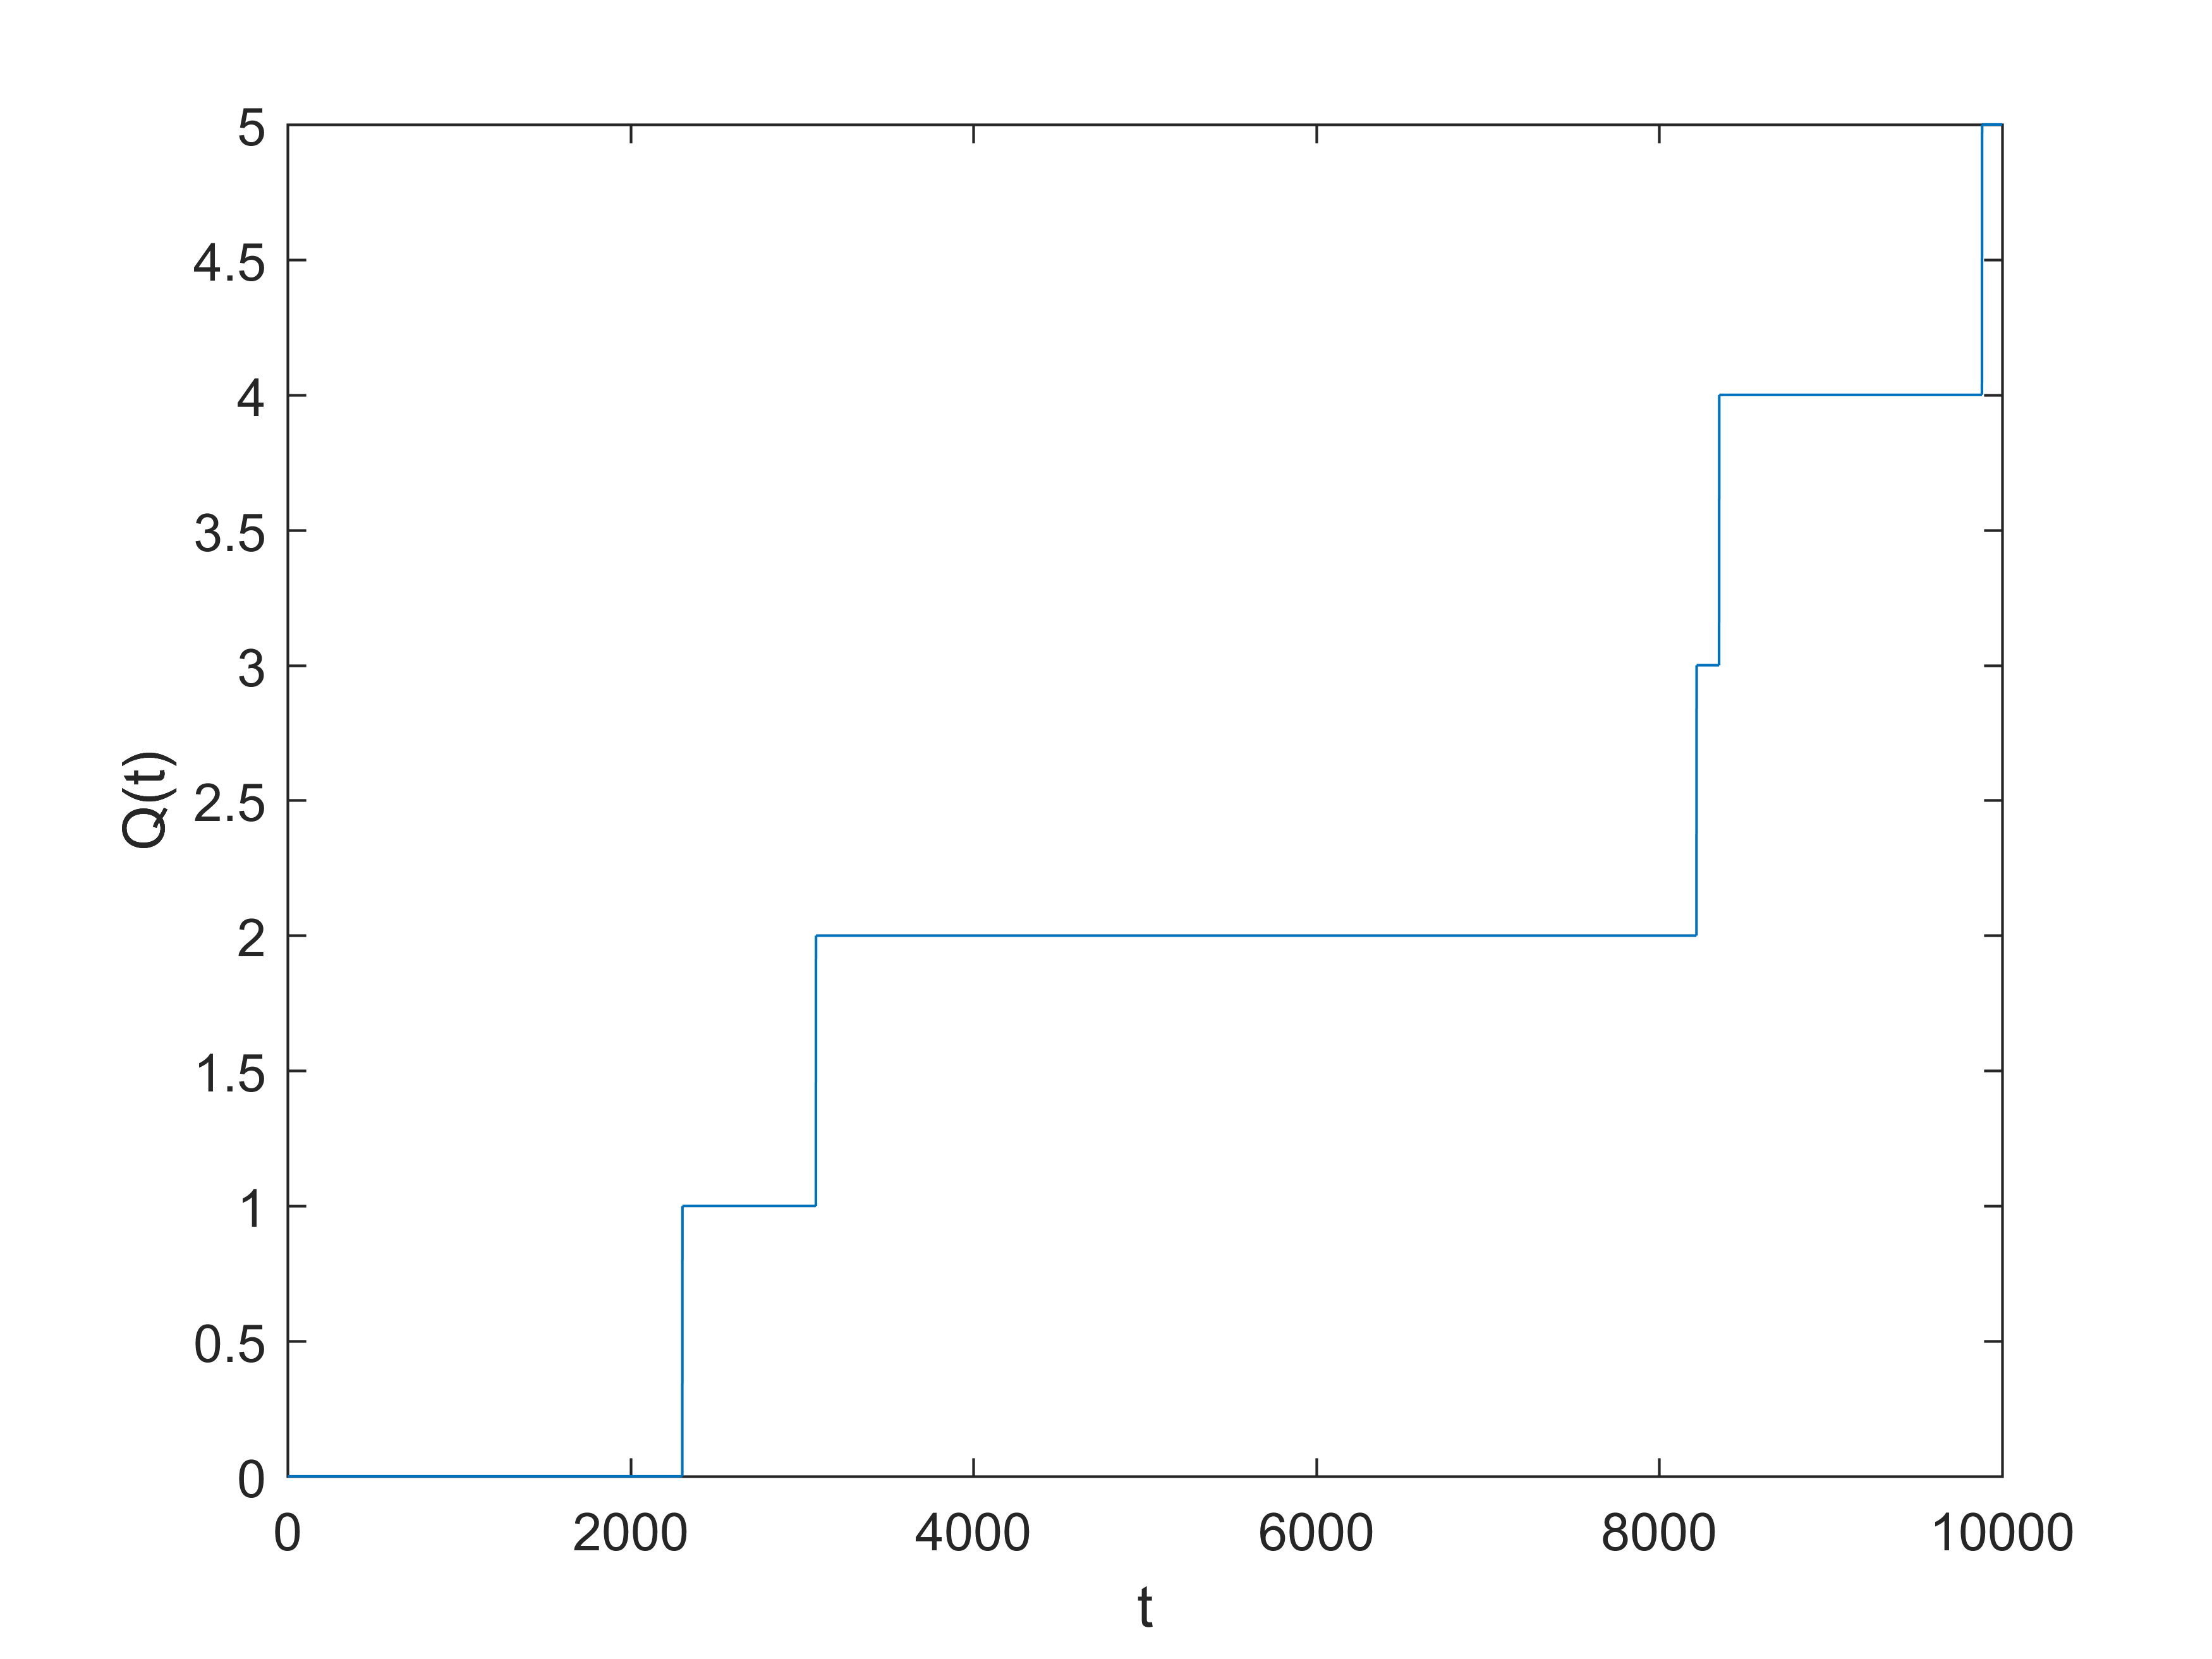
\includegraphics[scale=0.55]{Imagenes/Q1.png}
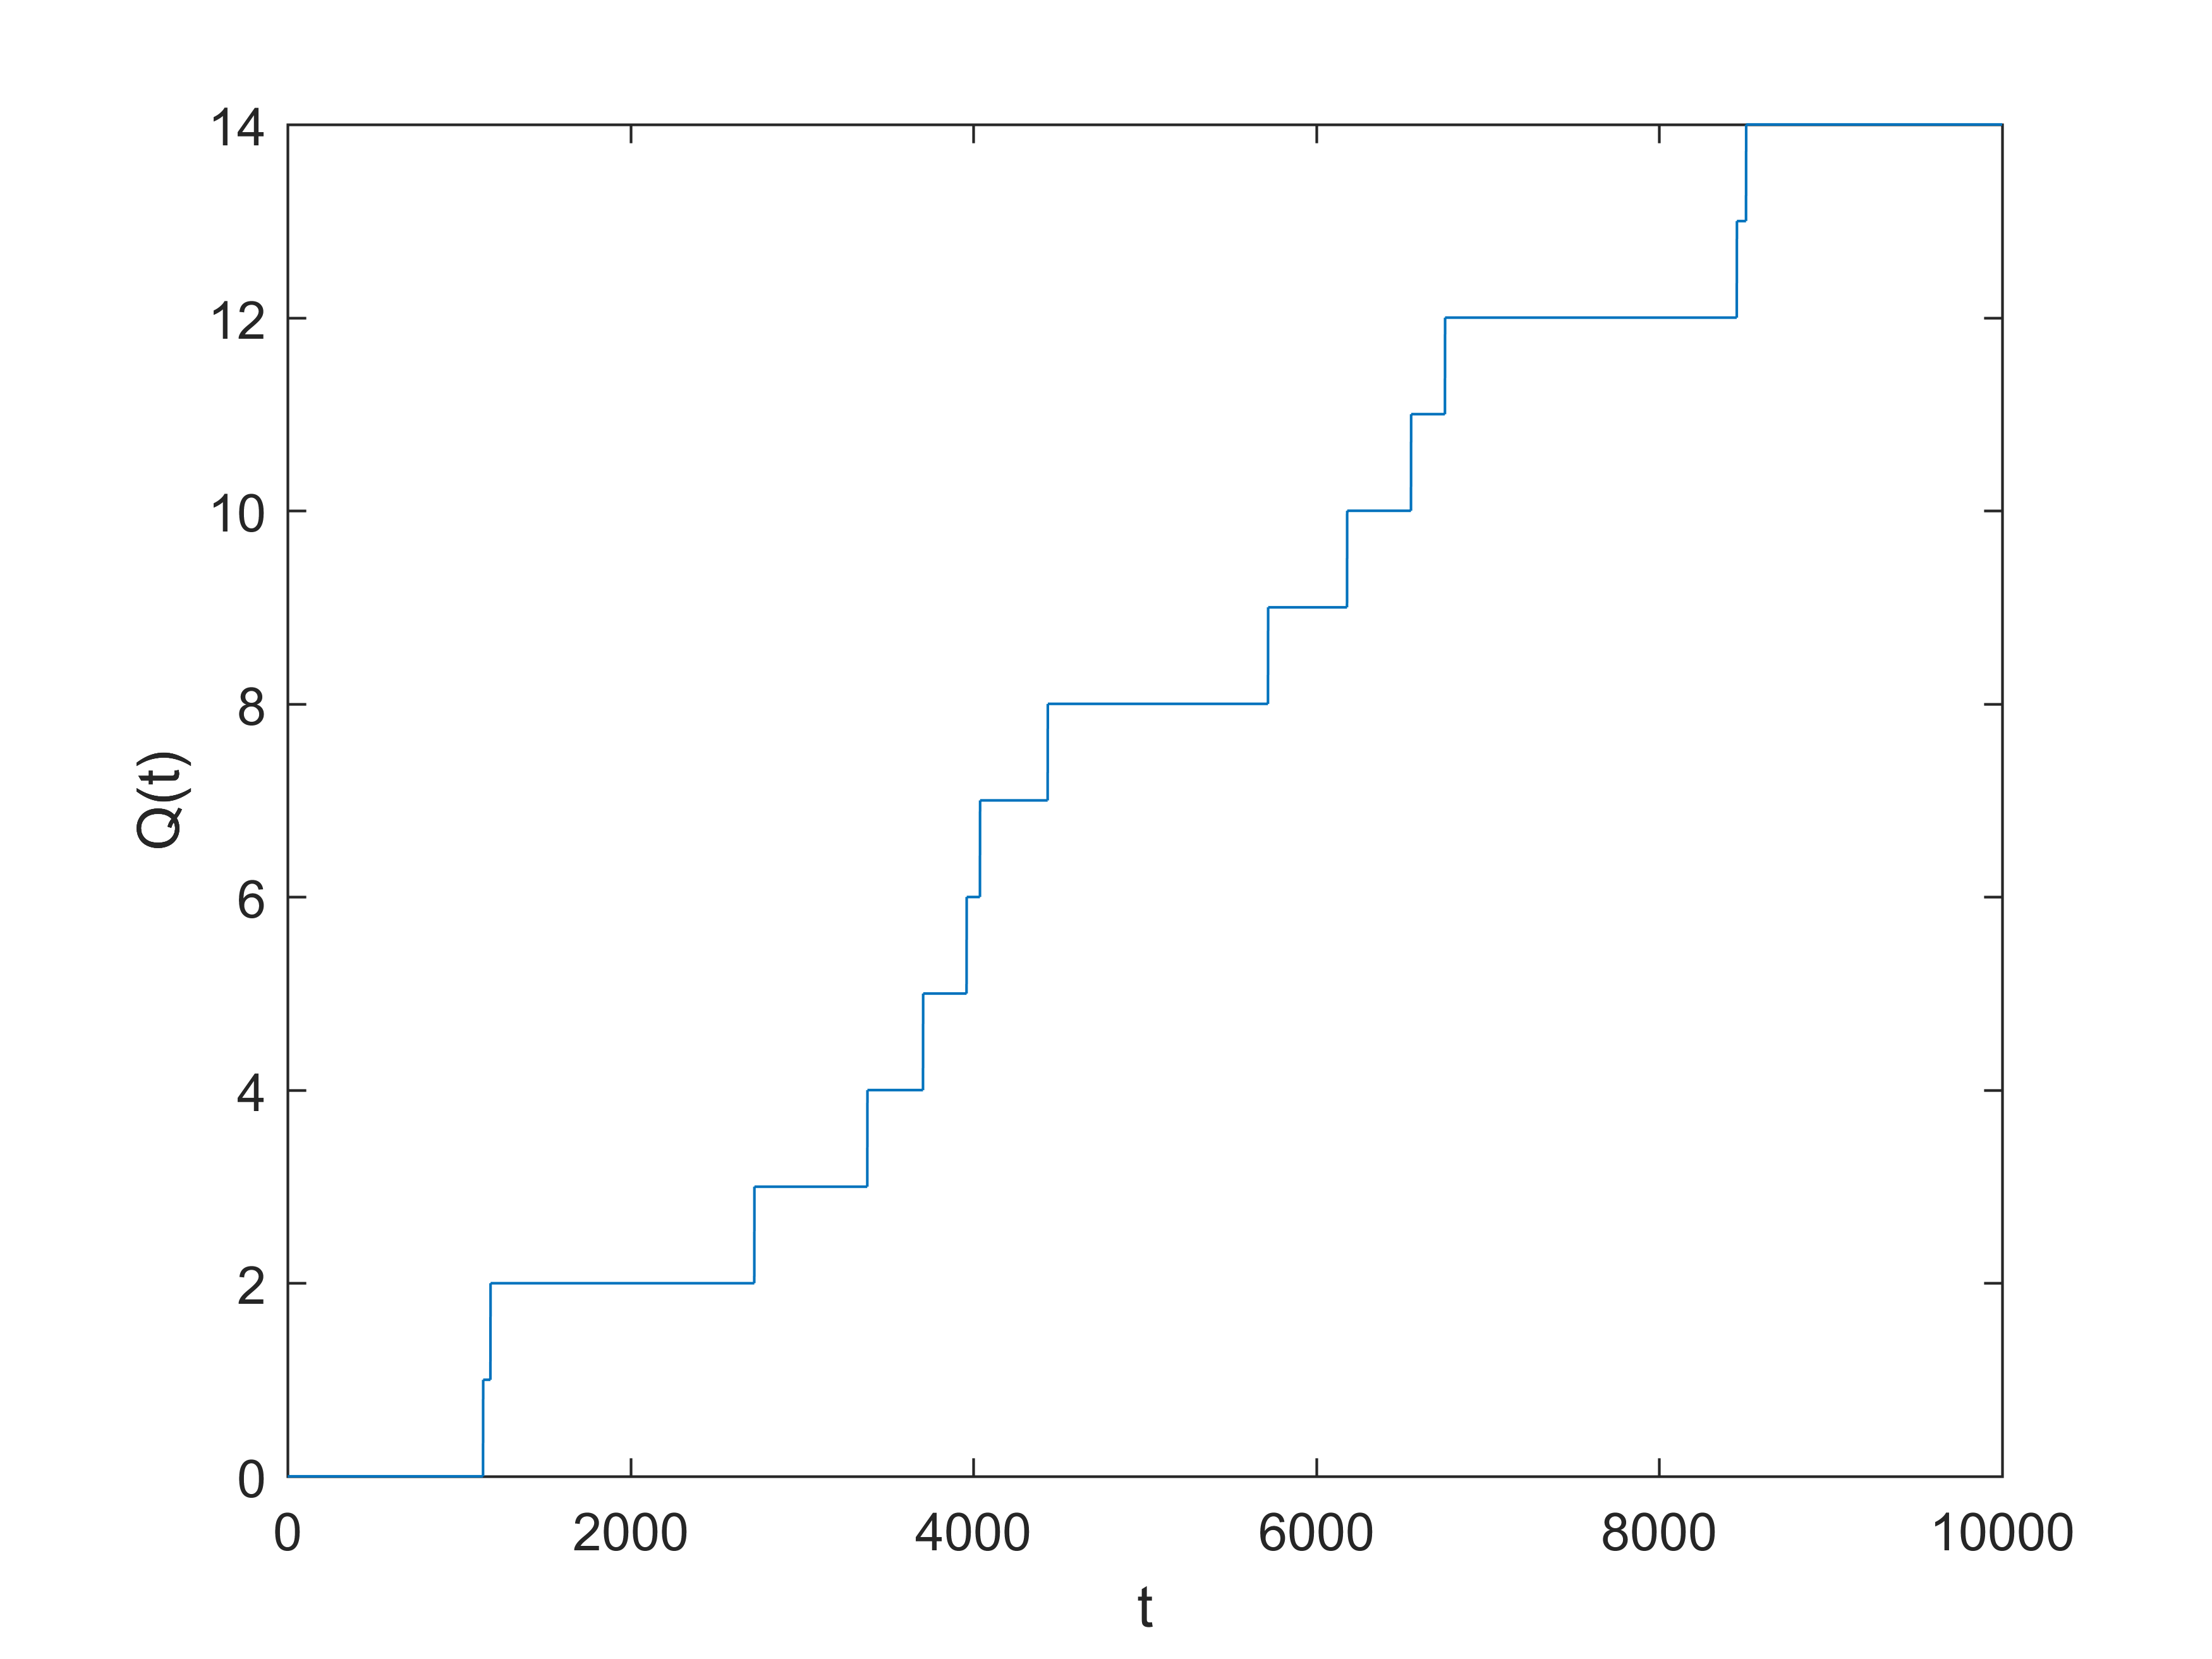
\includegraphics[scale=0.55]{Imagenes/Q2.png}
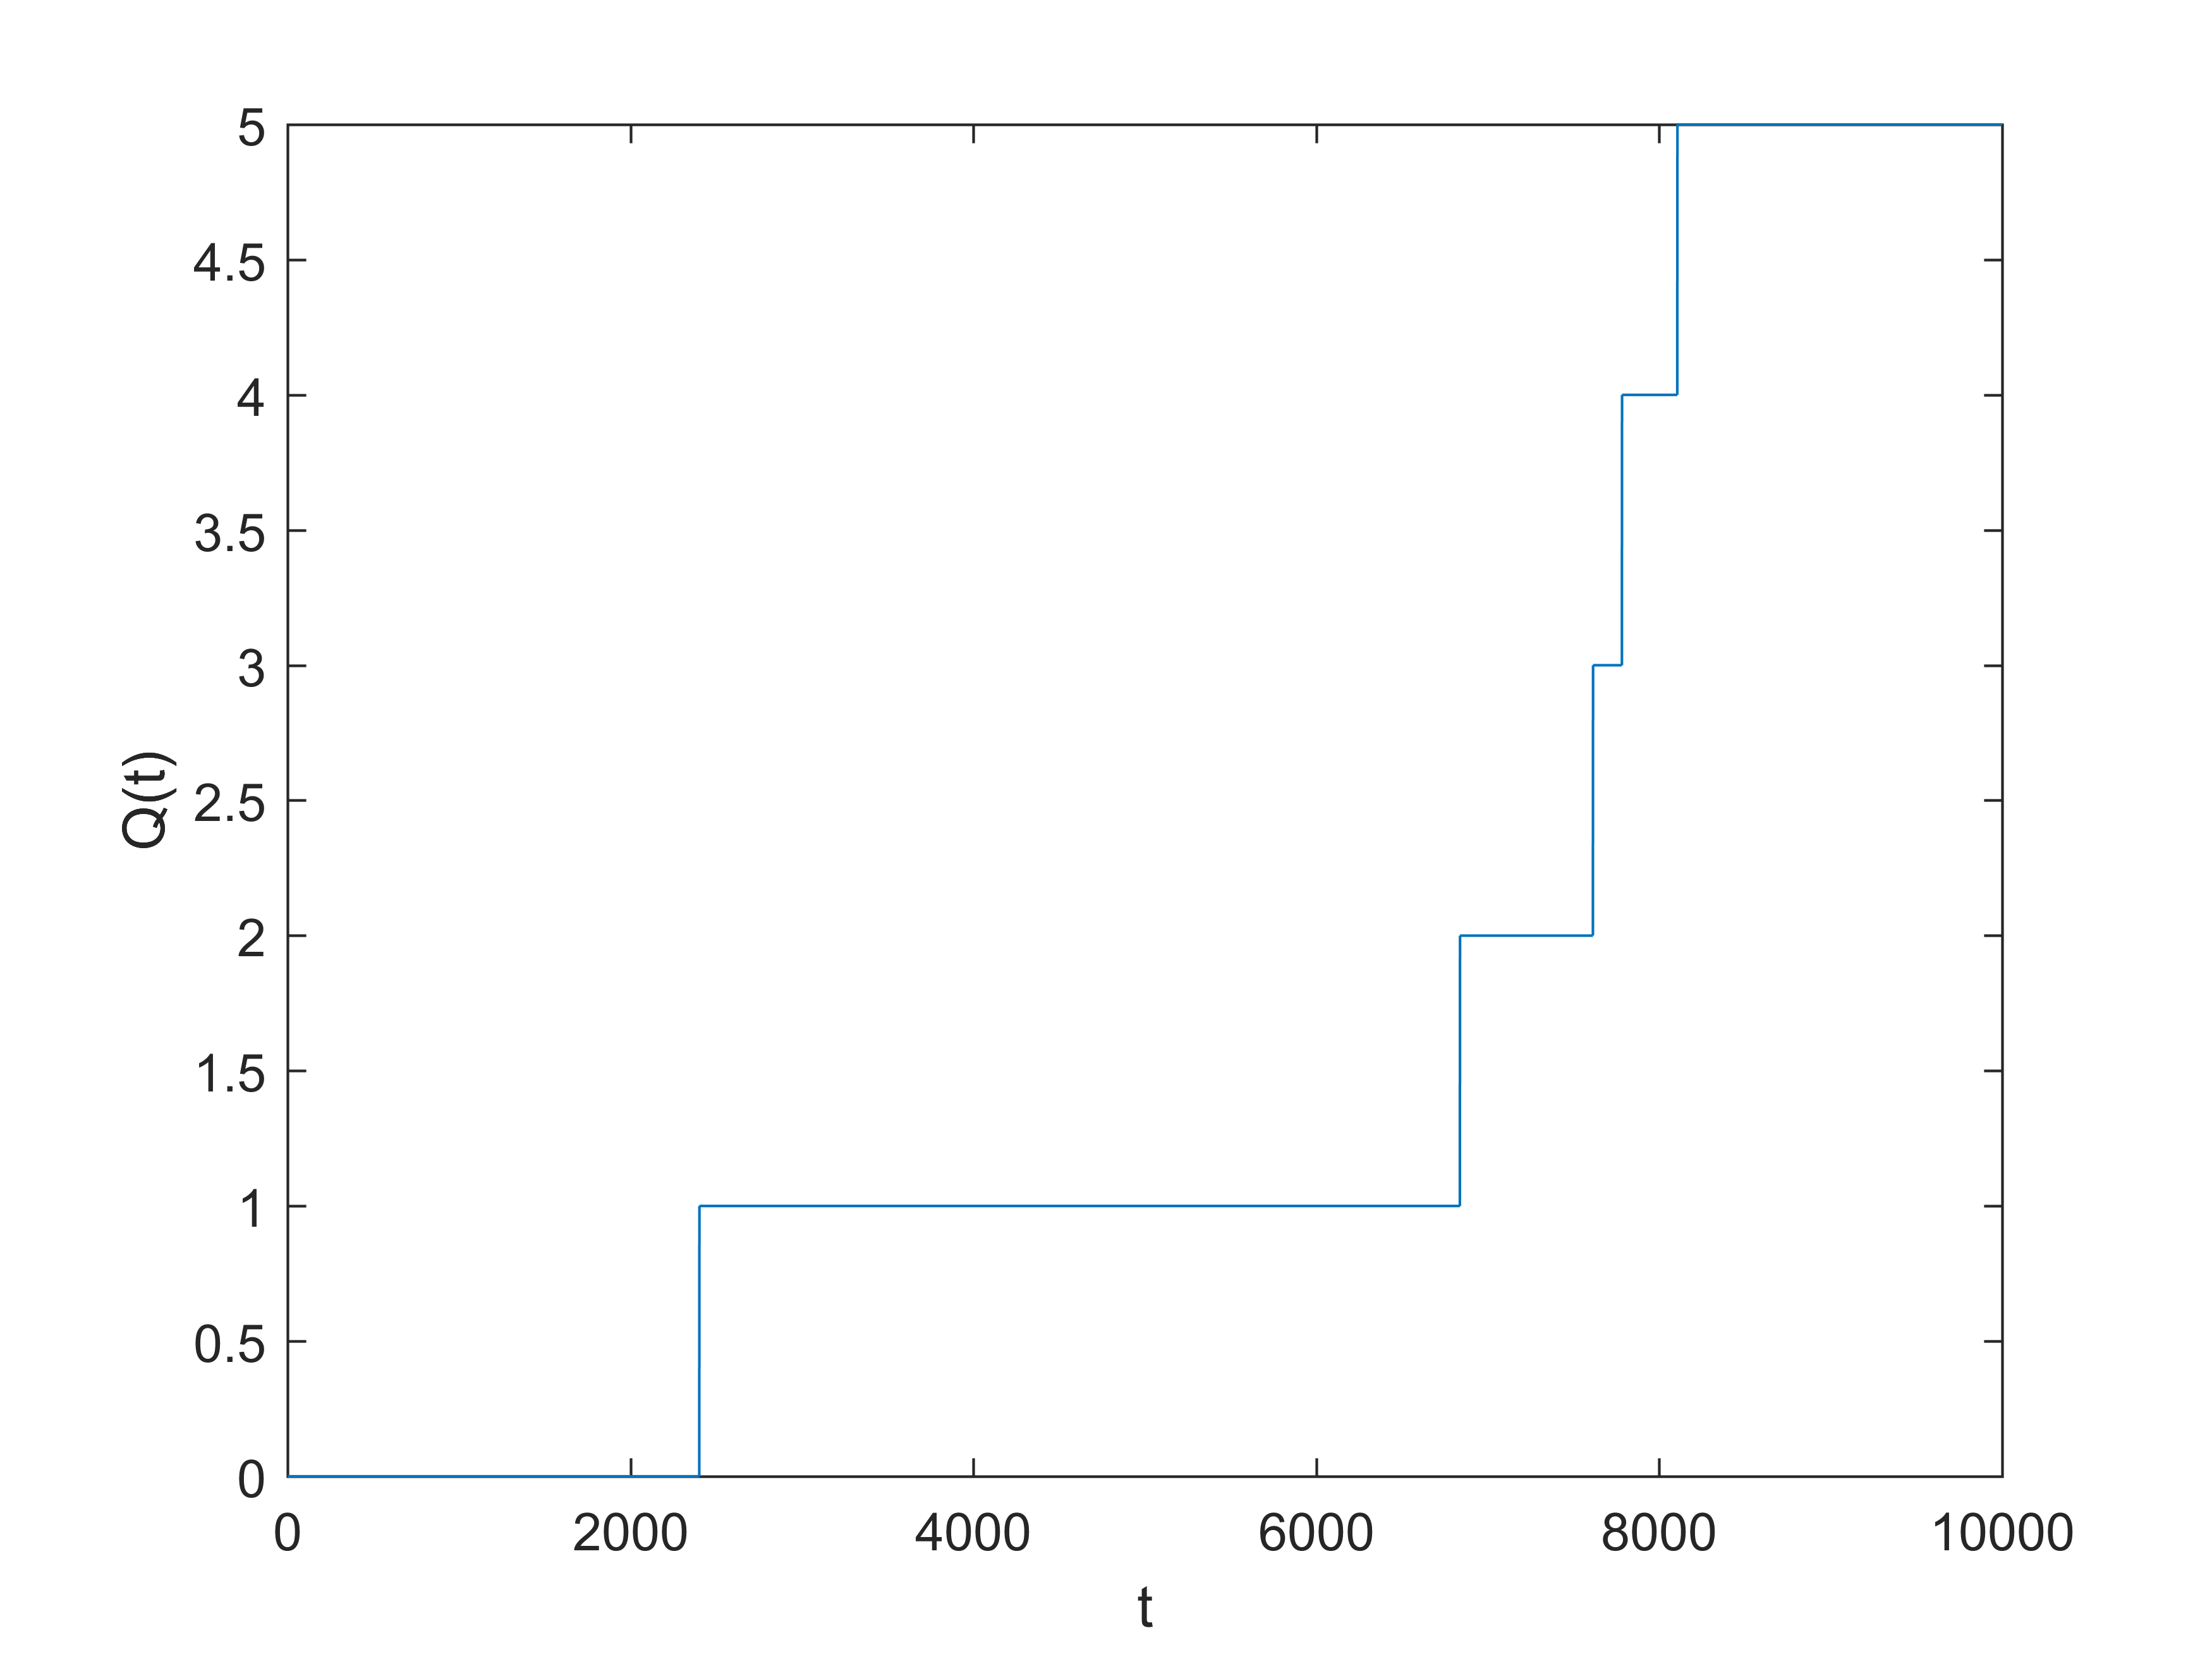
\includegraphics[scale=0.55]{Imagenes/Q3.png}
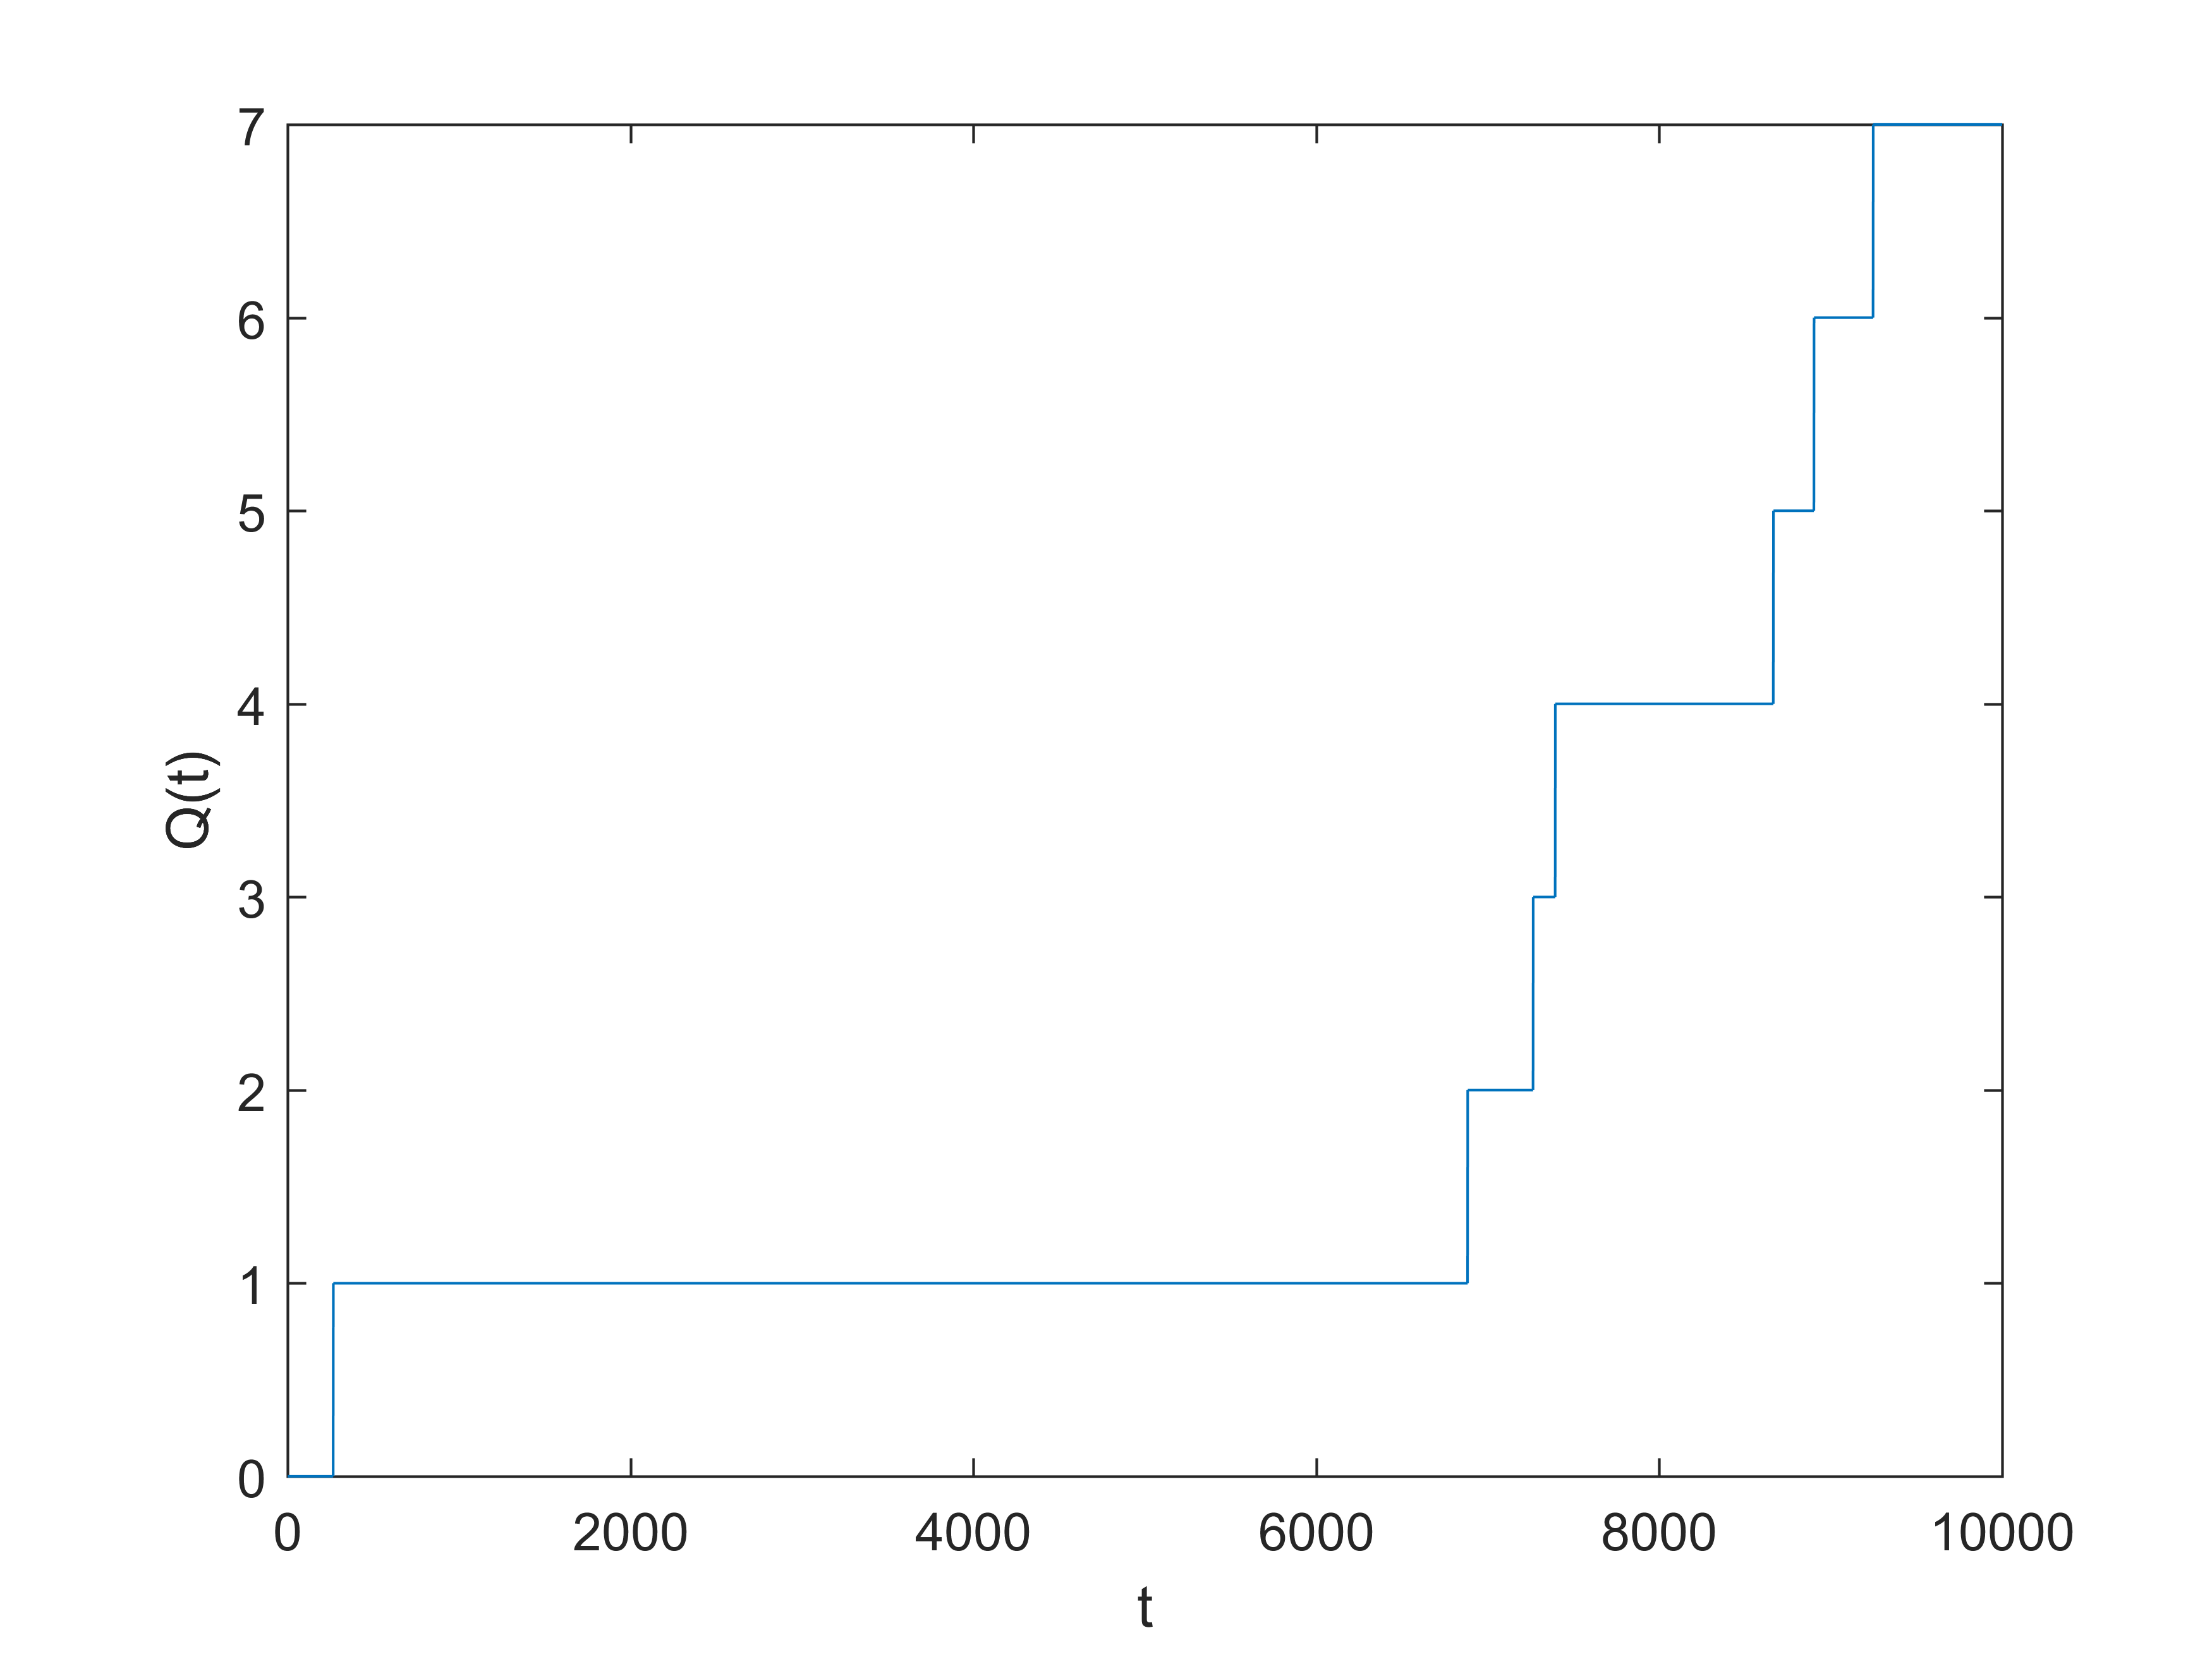
\includegraphics[scale=0.55]{Imagenes/Q4.png}
\par\end{centering}
\caption{Algunas funciones muestra generadas}

\end{figure} 

\newpage 

\subsection{C\'alculo de par\'ametros espec\'ificos}

Teniendo en cuenta el valor te\'orico de $\lambda = 1$ (y que $t_1 < t_2$), se calculan algunos par\'ametros en particular:

\[
E[Q(t)] = \lambda t \Longrightarrow E[Q(4)] = 4
\]
\[
\sigma^2[Q(t)] = \lambda t \Longrightarrow \sigma^2[Q(7)] = 7
\]
\[
R_{QQ}(t_1,t_2) = \lambda^2t_1t_2 + \lambda t_1 \Longrightarrow R_{QQ}(5,8) = 45
\]
\[
C_{QQ}(t_1,t_2) = R_{QQ}(t_1,t_2) - E[Q(t_1)] \cdot E[Q(t_2)] \Longrightarrow r_{QQ}(t_1,t_2) = \frac{C_{QQ}(t_1,t_2)}{\sqrt{C_{QQ}(t_1,t_1) \cdot C_{QQ}(t_2,t_2)}} \Longrightarrow r_{QQ}(2,3) = 0.8165
\]

Se comparan los valores te\'oricos con los simulados durante una corrida en el siguiente cuadro.

\begin{table}[ht]
\begin{centering}
\begin{tabular}{|c||c|c|}
\hline 
 & Te\'orico & Simulado\\
\hline 
\hline 
$E[Q(4)]$ & 4 & 4.0520\\
\hline 
$\sigma^2[Q(7)]$ & 7 & 6.8203\\
\hline 
$R_{QQ}(5,8)$ & 45 & 45.6080\\
\hline 
$r_{QQ}(2,3)$ & 0.8165 & 0.8024\\
\hline 
\end{tabular}
\par\end{centering}
\caption{Comparaci\'on de los par\'ametros obtenidos}

\end{table}

El c\'odigo utilizado para simular dichos valores se muestra a continuaci\'on. Se utilizaron para ello 1000 funciones muestra (N) de 10000 valores cada una (T), donde en cada caso el valor de $t$ corresponde a $t \cdot N$.

\lstinputlisting[language=Matlab, caption=C\'odigo de implementaci\'on]{Codigos/EJ3B.m}

\newpage

\subsection{Estimaci\'on de par\'ametros por promedio temporal}

Para ver si es posible estimar los par\'ametros anteriores realizando un promedio temporal sobre alguna de las funciones muestra (en lugar de hacerlo sobre el ensamble),se debe verificar que se cumplan ciertos requerimientos. Se considera el promedio temporal en tiempo continuo:

\[
<g[x(t)]>_T = \frac{1}{T} \int^{\frac{T}{2}}_{-\frac{T}{2}} g[x(t)] \; dt
\]

Para estimar la media con promedio temporal, debe resultar ser un proceso erg\'odico en la media. Para ello, debe cumplirse que:

\[
\underset{T \rightarrow \infty}{lim} E[<x(t)>_T] = \mu_x \hspace{2cm} \underset{T \rightarrow \infty}{lim} \sigma^2[<x(t)>_T] = 0
\]

Intuitivamente, se puede observar que no resultar\'a erg\'odico en la media sin realizar los c\'alculos, dado que si se toma una funci\'on $Q(t)$ cualquiera del ensamble, si $T \rightarrow \infty$ en el peor caso resulta que $Q(t) \rightarrow \infty$, dado que es mon\'otona creciente, por lo que el promedio tendre\'a a $\infty$. Se considera en este caso la integral desde 0 hasta T, dado que no hay tiempo negativo. Verificando la primera condici\'on:

\[
\underset{T \rightarrow \infty}{lim} \frac{1}{T} \int^{T}_{0} E[Q(t)] \; dt = \underset{T \rightarrow \infty}{lim} \frac{1}{T} \int^{T}_{0} \lambda t \; dt = \underset{T \rightarrow \infty}{lim} \frac{1}{T} \cdot \lambda \cdot \frac{T^2}{2} = \infty
\]

Por lo tanto, no puede estimarse la media mediante promedio temporal sobre una $Q(t)$ cualquiera del ensamble.\par
Para estimar la autocorrelaci\'on con promedio temporal, debe resultar un proceso erg\'odico en la autocorrelaci\'on. Para esto debe verificarse que:

\[
\underset{T \rightarrow \infty}{lim} E[<R_{xx}(t)>_T] = R_{xx}(t) \hspace{2cm} \underset{T \rightarrow \infty}{lim} \sigma^2[<R_{xx}(t)>_T] = \frac{1}{T} \int^{T}_{-T} \left( 1-\frac{|\tau|}{T} \right) C_{zz}(\tau) \; d\tau
\]
\par
Donde:

\[
z(t) = x(t) \cdot x(t+\tau) 
\]

En la expresi\'on de $R_{QQ}(t_1,t_2)$ hallada anteriormente, se observa que depende de los tiempos en cuesti\'on y no de la diferencia, por lo que el proceso no resulta erg\'odico en la autocorrelaci\'on. En consecuencia, no podr\'a estimarse tampoco mediante el promedio temporal de una funci\'on de muestra $Q(t)$ cualquiera del ensamble.

\end{document}